\chapter{Theory}\label{chapter:theory}

\section{Ball Screw Drive}
As shown in fig. \ref{fig:Ball_Screw} ball screws consist of five main components, the steel balls, screw shaft, nuts, seals, and tube. The steel balls serve as ball bearing between the screw shaft and the nuts. The screw shaft is mounted by fixed and free bearings is actuated by a motor. The nuts, which typically carry the load, move linearly along the screw shaft when the shaft is rotating. While the steel balls are rotated under external load and friction, the ball screw shaft is under constant compressive stress. Defects usually occur in the grooves of the screw shaft, guiding the steel balls, and the steel balls, which are subject to rolling friction. Defects usually start with little defects occurring on the surface of the ball screw shaft. When continuing to rotate the ball screw shaft, the system repetitively takes shocks each time the steel balls pass the surface defects. Depending on the location and severity of the defects the periodicity as well as the intensity of the shock varies. For this reason analysing recorded vibration signals seems promising for PHM systems \cite{Lee2015}. Of course surface defects also lower the efficiency of the system. Exemplary, one can imagine that the reduced efficiency leads to an increased demand of motor torque to move the load with the same speed and acceleration. This might become visible when looking at the electrical current of the motor. For this reason, also investigating the control signals of the industrial machine might be a good indicator for PHM systems.

\begin{figure}[H]
  \centering
  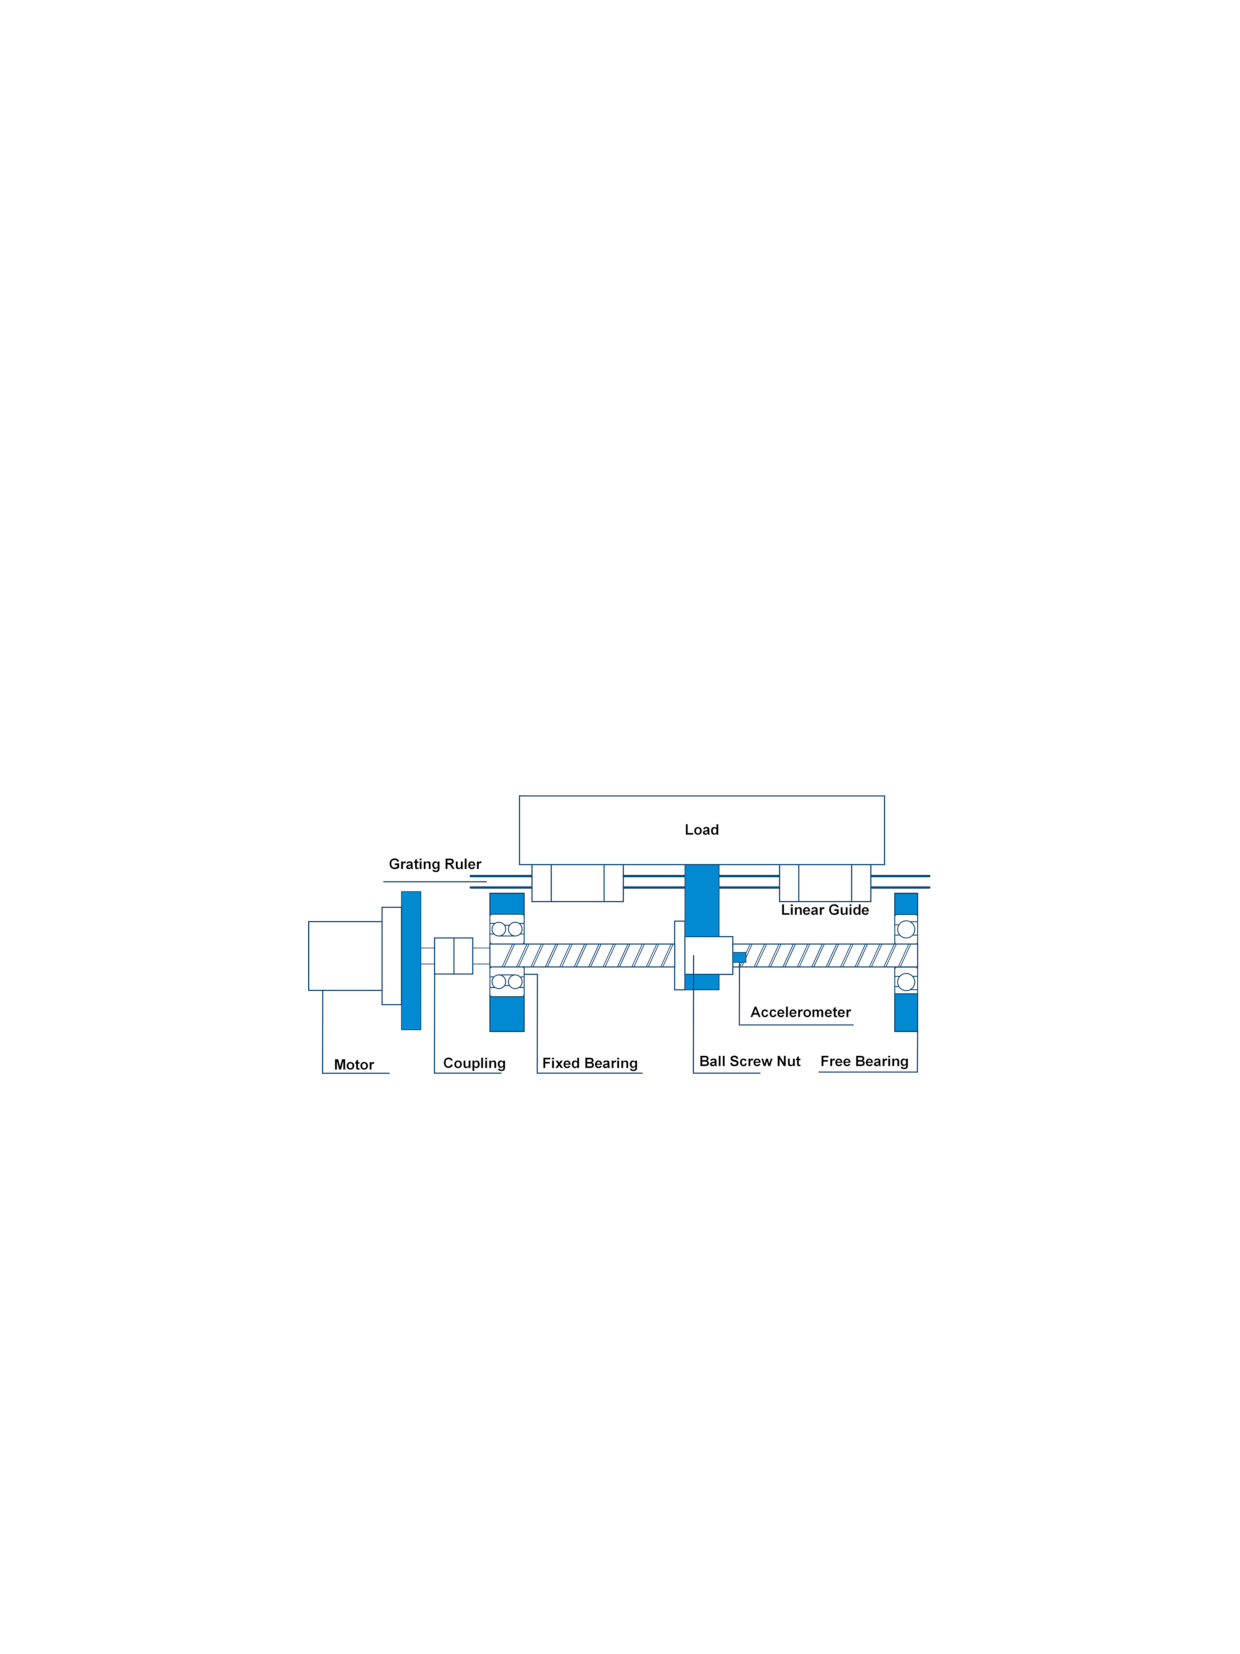
\includegraphics[width=1\textwidth]{Ball_Screw.pdf}
  \caption {Ball Screw Drive \cite{DENG2020}} \label{fig:Ball_Screw}
\end{figure}

\section{Neural Network}
The big data ecosystem is constantly evolving, and new technologies are coming up continuously, with many of them reacting more and more to the demands of the industry. Big data refers to an increasing volume of unstructured data, high sampling rates and a variety of different data sources. Modern technologies become relevant when processing this data to retrieve useful information. Machine learning is a research domain of algorithms that can recognize patterns in existing datasets by automatically evolving features during a training process. Deep Learning is a specific branch of machine learning. Inspired by the nature, neural networks try to imitate the function of human brains. The increased amount of data and computational power makes deep learning applications more attractive for real world use. Neural networks are hierarchically structured non-linear processing layers which try to learn hierarchical representations of data. Due to the increasing interest, the deep learning community recently came up with various new deep learning architectures. In the following, some of those are explained more in detail.

\subsection{Neural Network Architecture}
Neural networks consist of neurons which are layered in a hierarchical architecture. The neurons of consecutive layers are connected through weights and biases. During the optimization of the model, the weights and biases are updated. Fig. \ref{fig:neural_network_overview} shows the organization of neurons in an architecture with fully-connected layers. Each neuron from layer i is connected with all neurons from layer i+1 and shares information with them.

\begin{figure}[H]
  \centering
  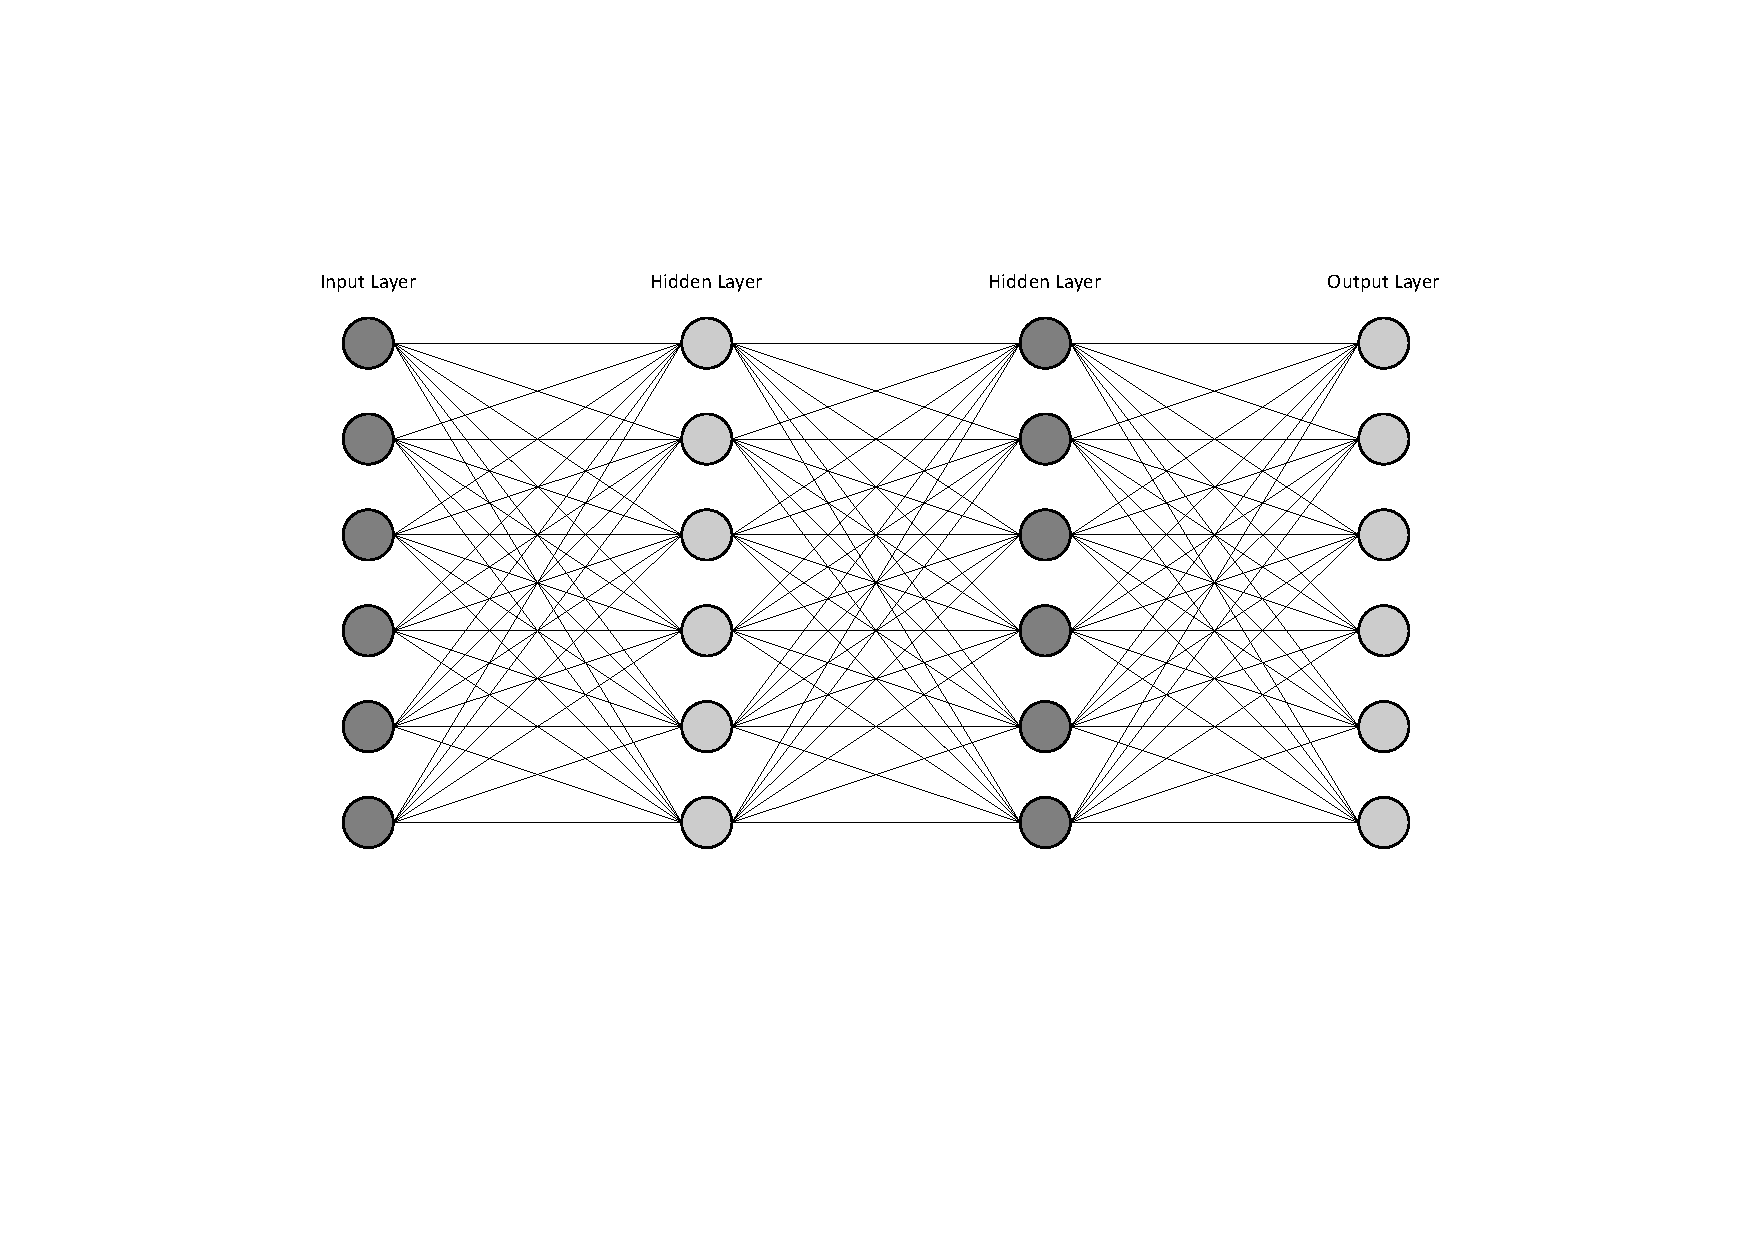
\includegraphics[width=0.7\textwidth]{neural_network_overview.pdf}
  \caption {Layer Overview Neural Network}
  \label{fig:neural_network_overview}
\end{figure}
The input of a neuron is calculated in two steps. Firstly, the weighted sum of all previous neuron's outputs and a bias is estimated. Afterwards, the result is processed by an activation function, which gives the neural network a non-linear property. Standard multilayer feedforward networks with even one single hidden layer and an arbitrary bounded and non-constant activation function are universal approximators. This means that a wide variety of functions can be represented by the neural network when given appropriate weights \cite{HORNIK1991}. Without activation functions, neural networks could only make linear assignments of inputs x to outputs y. With rising data complexity, the demand for a "non-linear" mapping from x to y is necessary. Without a non-linearity, the set of learnable functions is identical for neural networks with several and one hidden layer. Such neural networks would not mathematically realize complex relationships in the data. Fig. \ref{fig:neural_network_optimization} shows the forward and backward pass in a neural network at the example of one single neuron. First, the outputs of the neurons $i$ from the previous layers $l-1$, which are connected with the neuron of interest $j$ in layer $l$, are multiplied with its weights and summed up together with a bias $b_{j}$. The resulting logits $z_{j}$ are then processed by the activation function $\phi$. Different activation functions can be used throughout the network. After passing several consecutive hidden layers, a loss function evaluates the prediction with the ground truth label in the end of the network.

\subsection{Activation Function}
Different problems and network layers require different activation functions. One typically uses tanh, sigmoid and ReLU activations in hidden layers and a linear, sigmoid and softmax function in the final layer \cite{Brownlee2021}. Linear final layers are restricted to regression problems, whereas sigmoid and softmax functions are used for classification problems. The sigmoid function is used for binary and softmax for multiclass classification. In general, the softmax function is an extension of the sigmoid function to the multiclass case, which can be proofed easily. The softmax and sigmoid functions normalize the network output to a probability distribution over the predicted output classes. Deciding for activation functions in the hidden layers does not follow such clear rules. All the mentioned functions have different characteristics, which lead to individual advantages and disadvantages. The sigmoid and tanh activation function squeeze the inputs in values between -1 and 1. Both functions can suffer from the vanishing gradient problem, since the derivative of these functions is close to zero for very big or small inputs. A solution for that is the ReLU activation function, which solves that problem but maps all negative inputs to zero. This so-called dead ReLU problem is solved by the Leaky Relu und ELU activation functions.  \cite{Brownlee2021}. In table \ref{tab:activation_functions} some of the most popular activation functions are described.

\begin {table}[H]
\begin{tabular}{ c c c c }
\toprule 
Formula & Formulation s(x) & Derivative $\frac{ds(x)}{dx}$ & Function Output Range \\
\midrule 
ReLU &   $\begin{cases} 0 & \text{, for }x < 0\\
	x & \text{, for }x \geqslant 0 \end{cases}$ & $\begin{cases} 0 & \text{, for }1 < 0\\
	1 & \text{, for }x \geqslant 0 \end{cases}$ & $[ 0, \infty)$\\

\rule{0pt}{5ex}%  EXTRA vertical height 

Leaky ReLU &   $\begin{cases} \alpha x & \text{, for }x < 0\\
	x & \text{, for }x \geqslant 0 \end{cases}$ & $\begin{cases} \alpha & \text{, for }1 < 0\\
	1 & \text{, for }x \geqslant 0 \end{cases}$ & $(- \infty, \infty)$\\

\rule{0pt}{5ex}%  EXTRA vertical height 

ELU &   $\begin{cases} \alpha(e^{x} - 1) & \text{, for }x < 0\\
	x & \text{, for }x \geqslant 0 \end{cases}$ & $\begin{cases} \alpha e^{x} & \text{, for }x < 0\\
	1 & \text{, for }x \geqslant 0 \end{cases}$ & $[ -\alpha, \infty)$\\
	
\rule{0pt}{5ex}%  EXTRA vertical height 
	
Sigmoid & $\frac{1}{1+e^{-x}}$ & $\frac{e^{-x}}{(1+e^{-x})^{2}}$ & (0,1)\\

\rule{0pt}{5ex}%  EXTRA vertical height 

Softmax & $\frac{e^{x_{i}}}{\sum_{j=1}^{K} e^{x_{j}}}$ & $\frac{e^{-x}}{(1+e^{-x})^{2}}$ & (0,1)\\

\rule{0pt}{5ex}%  EXTRA vertical height 

tanh & $\frac{e^{2x}-1}{e^{2x}+1}$ & $1-tanh^{2}(x)$ & $(-1,1)$ \\
\bottomrule  

\end{tabular}
\caption {Overview Activation Functions} \label{tab:activation_functions}
\end {table}
\subsection{Optimization}
When training neural networks one has to decide for a loss function and an optimizer. 

\subsubsection{Loss}
The loss function acts as a model evaluation criterion and the optimizer is responsible for changing the model according to the criterion. Deep learning can be applied in two different use cases: (1) regression tasks and (2) classification tasks. In a regression problem, the goal is to learn a mapping function from input variables to a continuous output variable. Contrariwise, in a classification problem, the model aims to predict a class label for each input sample \cite{ShilohPerl2020}. Typically, the mean square error (MSE) is applied as criterion in regression tasks:

\begin{equation}
L(X) =  \sum_{x}(\hat{y}(x)-y(x))^2,
\end{equation}

where $y(x)$ is the ground truth and $\hat{y}(x)$ the predicted class label \cite{ShilohPerl2020}. On the other hand, a Cross Entropy Loss is common for classification tasks: 

\begin{equation}
L(X) = \sum_{x} y(x) log(p(x)),
\end{equation}
where p(x) is the predicted probability of the sample $x$ belonging to the ground truth class $y(x)$ \cite{ShilohPerl2020}.

\subsection{Training Loop}
During training, the model's weights and biases need to be adapted such that the criterion is minimized. This optimization takes place in a two stage process:
\begin{itemize}
    \item \textbf{Forward Pass}: Calculating the neuron values throughout the network and the loss from the model prediction and the ground truth values or classes.
    \item \textbf{Backward Pass}: Calculating the derivative of the criterion with respect to the model parameter and updating those to reduce the loss.
\end{itemize}
Iteratively, these two steps are performed to optimize the model. The process is visualized in fig. \ref{fig:neural_network_optimization}. By calculating the partial derivatives of each layer and concatenating them in a reverse order of the forward pass, the gradients used for updating the model parameters can be established. For concatenating the partial derivatives, the chain rule is used:
\begin{equation}
 \frac{\delta L_{i}}{\delta w_{i}} = \frac{\delta L_{i}}{\delta \hat{y_{i}}} * \frac{\delta \hat{y_{i}}}{\delta z_{i}} * \frac{\delta z_{i}}{\delta w_{i}}, 
 \label{chain_rule}
\end{equation}
where $\frac{\delta L_{i}}{\delta \hat{y_{i}}}$ is the derivative of the loss with respect to the activation in the final layer, $\frac{\delta \hat{y_{i}}}{\delta z_{i}}$ is the derivative of the used activation function.  $\frac{\delta z_{i}}{\delta w_{i}}$ is the derivative of the logits $z_{i}$ with respect to the weights and biases used between the last two layers of the network \cite{ShilohPerl2020}. The gradients for all the previous layers needs to be estimated and concatenated equally to update all parameters in the model.

\begin{figure}[H]
  \centering
  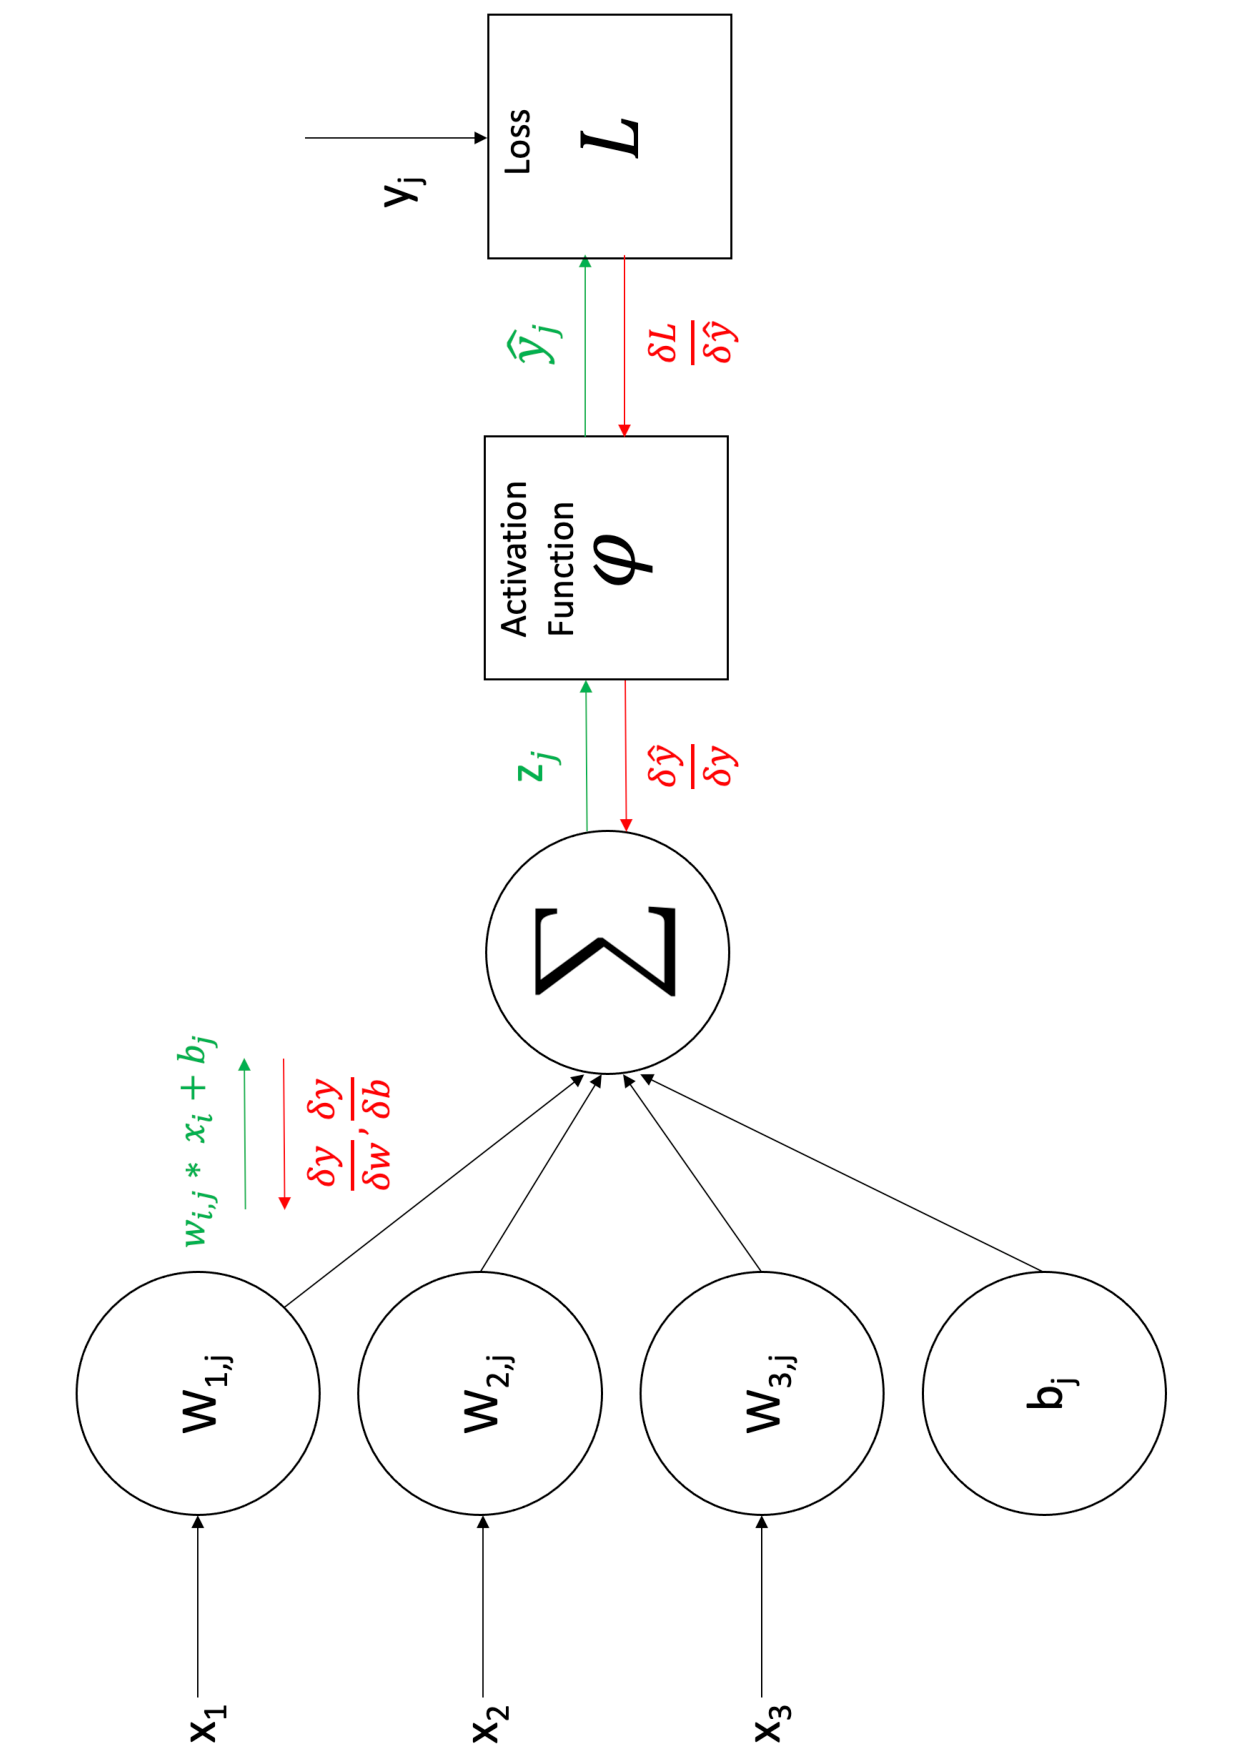
\includegraphics[width=0.7\textwidth]{neural_network_optimization.pdf}
  \caption {Optimization of Neural Network}
  \label{fig:neural_network_optimization}
\end{figure}

\subsection{Optimizer}
Calculating the gradient for the whole dataset is computationally expensive. A common practice is therefore to separate the dataset in several subsets, so called mini-batches. For each mini-batch, the gradients are calculated and the model is updated. This process is repeated for all the mini-batches retrieved from the dataset. Each training loop including the whole dataset is called an epoch. As soon as the loss converges the training can be terminated. Despite convergence, an optimal solution is not assured since the most neural network problems are not convex \cite{ShilohPerl2020}.

Most optimization methods are first order methods, which rely on gradients to update the model parameters. Second-order methods combine second and first order derivatives, which generally makes the method converge faster. These methods require the computation of the Hessian, which is especially expansive for big datasets and models. Also, first order methods can suffer from long training times when calculating gradients for big datasets (batch gradient descent). A method which tries to circumnavigate this problem is the Stochastic Gradient Descent (SGD). Repetitively, the model is updated with gradients based on a single sample, which is picked randomly from the dataset. Since the choice of these samples is random, the optimization suffers from instability and fluctuation. The mini-batch gradient descent is a compromise between the regular SGD and batch gradient descent. The gradient and model update is neither performed for a single sample nor for the whole dataset. It is performed on a small and randomly picked subset of the data, which accelerates the convergence of the training.
In order to accelerate and stabilize the optimization, one can also include historical gradients and update the model weights with a moving average over the past gradients. First and second order momenta are methods which accelerate SGD in the relevant direction and dampens oscillations \cite{ShilohPerl2020}. This variant of the regular gradient descent allows an optimization with an adaptive step size in the different dimensions of the latent feature space. To learn faster, the step size can be increased in the relevant and decreased in the irrelevant directions. Each training loop including the whole dataset is called an epoch. As soon as the loss converges, the training can be terminated. Despite convergence an optimal solution is not assured since the most neural network problems are not convex \cite{ShilohPerl2020}.\newline\newline

\textbf{Momentum}
Updating the model parameters with momentum is a procedure which includes two steps. In a first step, the moving average over the past gradients is calculated and in a second step the model parameters are updated accordingly:

\begin{equation}
  \begin{aligned}
      v_{t} = & \gamma v_{t-1} +  \eta \nabla_{\theta}L(W_{t-1}) &\\
      W_{t} = &W_{t-1} - v_{t},
      \label{eqn:momentum}
  \end{aligned}
\end{equation}

where $v_{t}$ is the updated and $v_{t-1}$ the current momentum, $W_{t}$ is the updated and $W_{t-1}$ the current model weights, $\nabla_{\theta}L(W_{t-1})$ is the derivative of the loss with respect to the current model weights, $\eta$ is the learning rate and $\gamma$ defines the relationship between the current momentum and gradient for calculating the updated momentum \cite{Ruder2016}.
\newline
\newline
\textbf{Nesterov Accelerated Gradient}
\newline
Another well known optimizer of this kind is Nesterov Accelerated Gradient (NAG), which extends the regular first order momentum update rules. When calculating the first order momentum, NAG calculates the gradient not with respect to the current but to the pre-updated weights: 

\begin{equation}
    \nabla_{\theta}L( W_{t-1} - \gamma v_{t-1}),
\end{equation}

where $W_{t-1}$ are the current model weights, which are pre-updated with the current first order momentum $v_{t-1}$. Just like described in equation \ref{eqn:momentum} the pre-updated gradient is used to calculate the updated momentum in a first step, which is then applied to update the model weights in a second step \cite{Ruder2016}.
\newline
\newline
\textbf{Adagrad}
\newline
Like all mentioned optimization methods also Adagrad is a gradient based optimization. Adagrad uses a squared version of the moving average over the past gradients:

\begin{equation}
  \begin{aligned}
  W_{t} = W_{t-1} - \frac{\eta}{\sqrt[2]{G_{t}+ \epsilon}} \bigodot \nabla_{\theta}L(W_{t-1}),
  \end{aligned}
  \label{eq:Adagrad}
\end{equation}

where  $W_{t-1}$ are the current and $W_{t}$ the updated model weights, $\nabla_{\theta}L(W_{t})$ is the derivative of the loss with respect to the current model weights. $G_{t}$ is the second order momentum, which is a diagonal matrix where each diagonal element i,i is the sum of the squares of the gradients with respect to the model parameter i up to time step t. $\epsilon$ denotes a small quantity which prevents the division by zero and $\gamma$ is the learning rate \cite{Ruder2016}.
\newline
\newline
\textbf{Adaptive Moment Estimation}
\newline
Adaptive Moment Estimation (Adam) is one of the most popular optimizer. ADAM combines the idea of first and second order momentum: 
\begin{equation}
  \begin{aligned}
   &m_{t} =  \beta_{1} m_{t-1} +  (1-\beta_{1}) \nabla_{\theta}L(W_{t-1}) &\\
    &v_{t} =  \beta_{2} v_{t-1} +  (1-\beta_{2}) \nabla_{\theta}L^{2}(W_{t-1}) &\\
    &\hat{m}_{t} = \frac{m_{t}}{1-\beta_{1}^{t}}&\\
    &\hat{v}_{t} = \frac{v_{t}}{1-\beta_{2}^{t}}&\\
   & W_{t} = W_{t-1} - \frac{\eta}{\sqrt[2]{\hat{v}_{t} + \epsilon}}\hat{m}_{t}, &\\
  \end{aligned}
  \label{eq:ADAM}
\end{equation}

where $m_{t}$ and $v_{t}$ are the first and second momentum, $\hat{m}_{t}$ and $\hat{v}_{t}$ are the bias-corrected first and second moment estimates, $\beta_{1}$ and $\beta_{2}$ are the weighting factors for the moving average and $W_{t-1}$ and  $W_{t}$ are the current and updated model weights \cite{Ruder2016}.

\section{Convolutional Neural Network}

Equally, to regular neural networks, convolutional neural networks (CNNs) consist of several neurons embedded in a fixed architecture. Developed for computer vision applications, the architecture of CNNs is optimized to process images. In CNNs the neurons are structured in layers just like in normal neural networks. In regular networks the neurons of one layer are organized in one dimension and in CNNs in three dimensions (height, width, depth). The functionality of CNNs is visualized in \ref{fig:CNN_overview}. One can identify four main compounds of a CNN, which are described more detailed in the following:

\begin{itemize}
    \item [1.] The input data is organized in a structured and grid-like form. Each element in this structure is called a pixel, which described by its specific value and position. The data is stored in arrays with spatial dimension (height x width) and depth (channel size).
    
    \item [2.] Convolutional layers contain kernels which are convolved with the input. The kernel contains weights and biases which are learned during training. An 'elementwise' activation function is applied to the kernel outputs.
    
    \item [3.]  Pooling layers downsample the spatial dimension. This reduces the height and width of the feature maps throughout the network. This minimizes the learnable network parameters.
    
    \item [4.] In the end fully-connected layers coupled with activation functions attempt to predict class labels for the input data.
\end{itemize}

\begin{figure}[H]
  \centering
  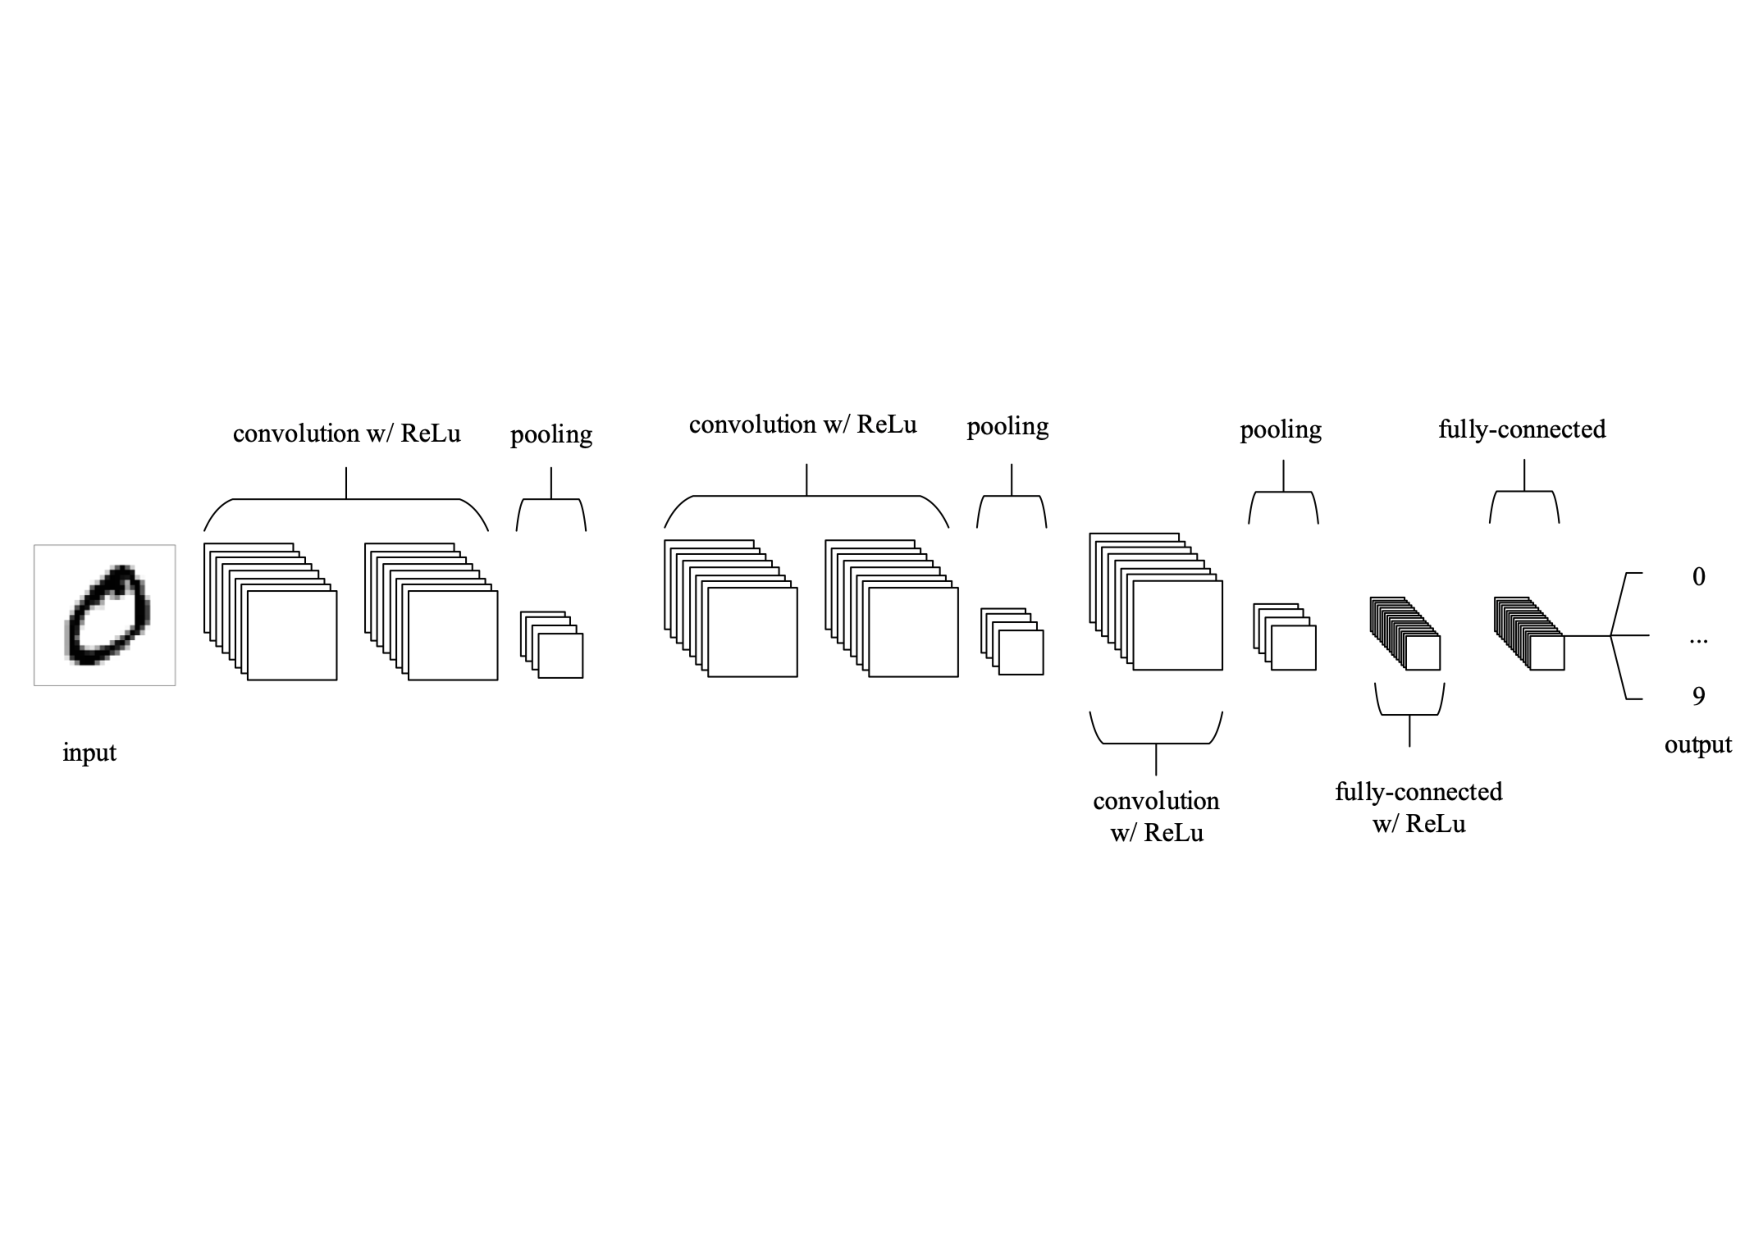
\includegraphics[width=0.9\textwidth]{cnn/cnn_architecture.pdf}
  \caption {Overview CNN Architectures \cite{OShea2015}}
  \label{fig:CNN_overview}
\end{figure}

In the following typical CNN layers are described more in detail. 

\subsection{Kernel}
The convolutional layers are the core elements in a CNN. The learnable parameters in a convolutional layer are the weights and biases of the kernel. During the optimization, each kernel learns to extract expressive features. The depth of a kernel is defined by the depth of the input layer and the number of applied kernels defines the depth of the subsequent feature map. Each channel corresponds to the features extracted by the convolution of a single kernel with the data across the whole spatial dimension. Usually, the spatial dimensions (width, height) are reduced and the depth of the latent feature map is increased throughout the network. Therefore, the network extracts more global features in the beginning and more local features in the end of the network.  \cite{OShea2015}. Looking at fig. \ref{fig:kernel_number} one can see how the kernel of depth 3 is applied to the input of depth 3. By using 6 kernels, the resulting feature map is of depth 6.

\begin{figure}[H]
  \centering
  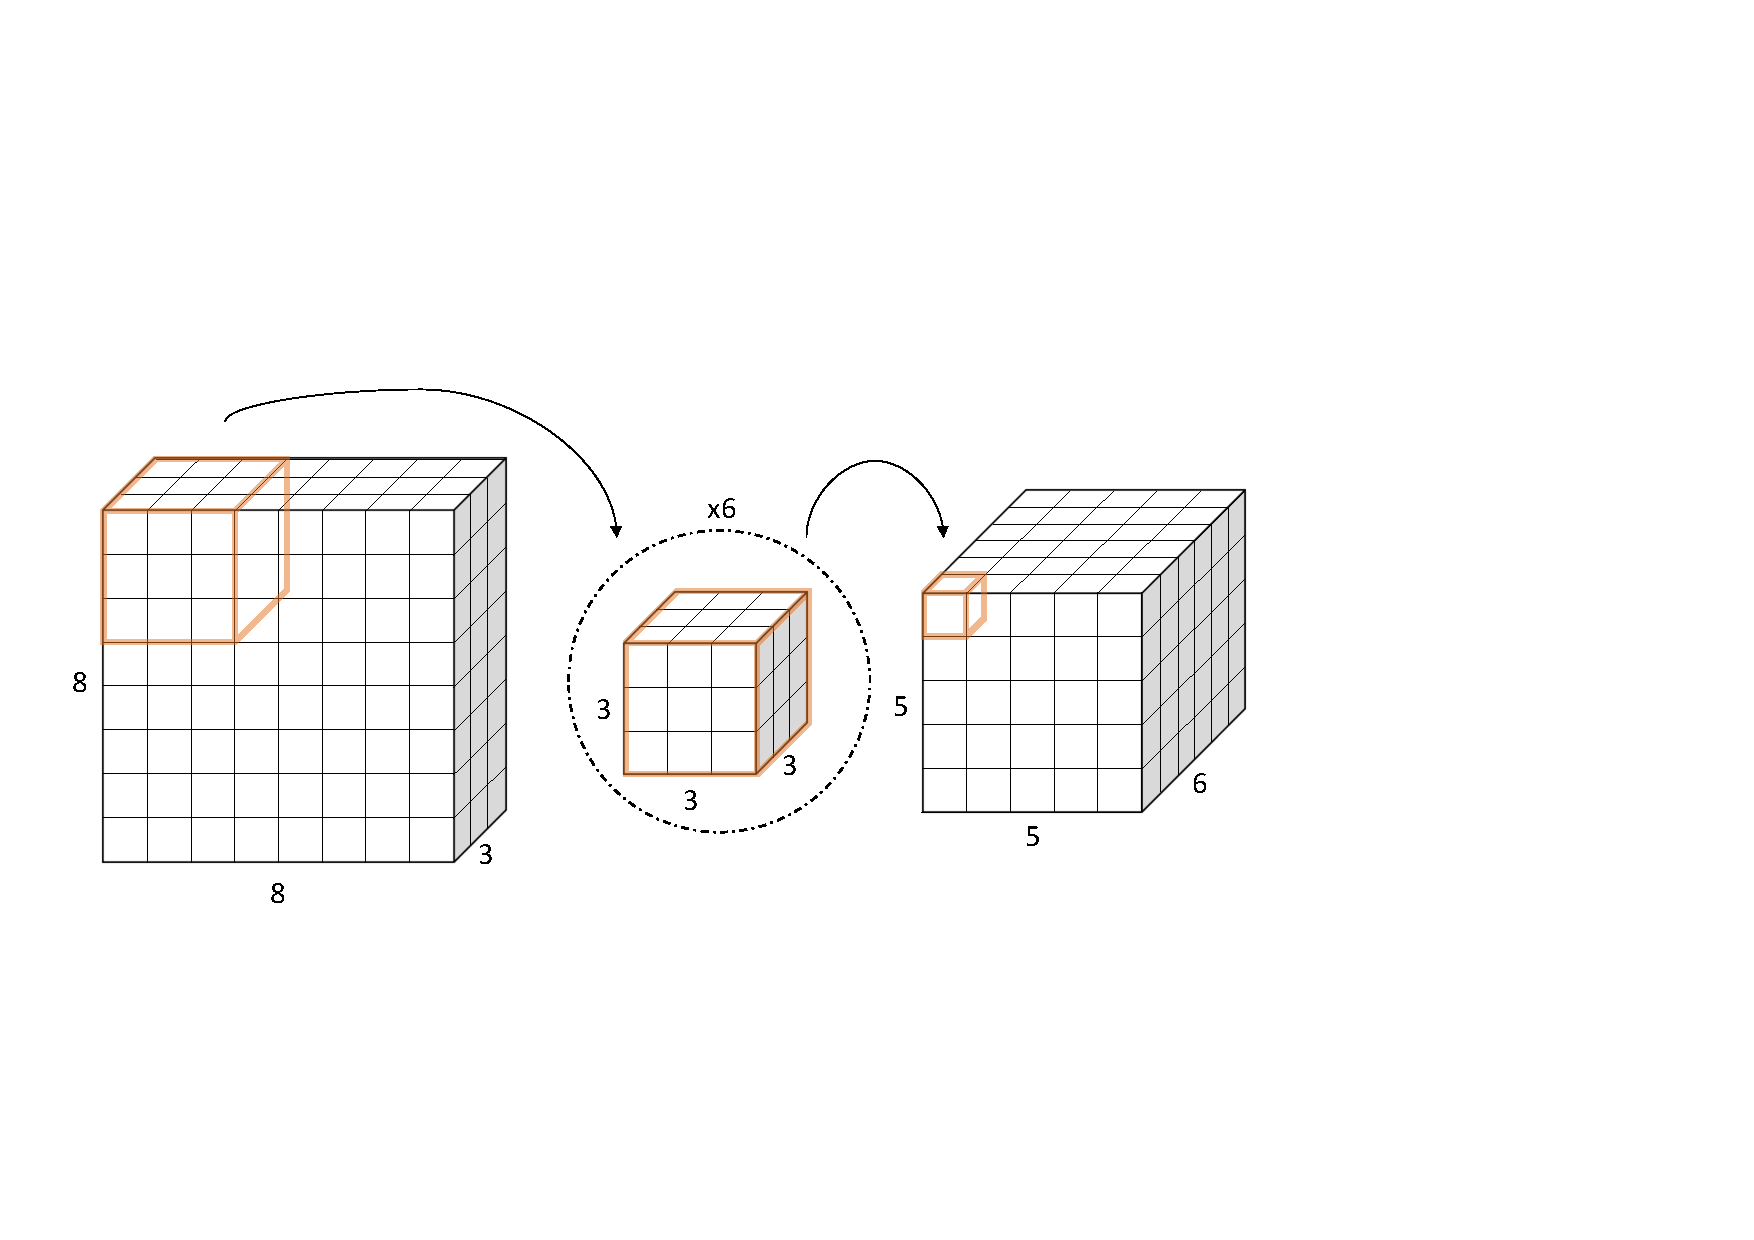
\includegraphics[width=0.6\textwidth]{cnn/kernel_number.pdf}
  \caption {2D Convolution with 6 Kernels of Depth 3 based on \cite{Ganesh2019}}
  \label{fig:kernel_number}
\end{figure}

To make things easier a single convolution of a kernel with a subspace of the input data is shown for the 1D case:

\begin{equation}
  y(p_{0}) = \sum_{p_{n} \in R} w(p_{n}) \cdot x(p_{0} + p_{n}), 
  \label{eq:kernel}
\end{equation}

where $p_{n}$ is one of the $R$ kernel cells, $p_{0}$ is the lower bound pixel position of the input subspace involved in the single convolutional operation. Each kernel cell is multiplied with a corresponding pixel in the input and the $R$ outputs are summed up in the pixel $p_{0}$ of the subsequent feature map \cite{Ganesh2019}. Typically, a bias value is included in this weighted sum and a non-linearity is applied consecutively. The convolutional process is also visualized in fig. \ref{fig:kernel}, where $p_{n}$ is one of the three cells within the kernel, $R$ is three in this case and $p_{1}$ marks the lower bound pixel position of the input feature map and the pixel which sums all the information from the convolution in the output feature map.


\begin{figure}[H]
  \centering
  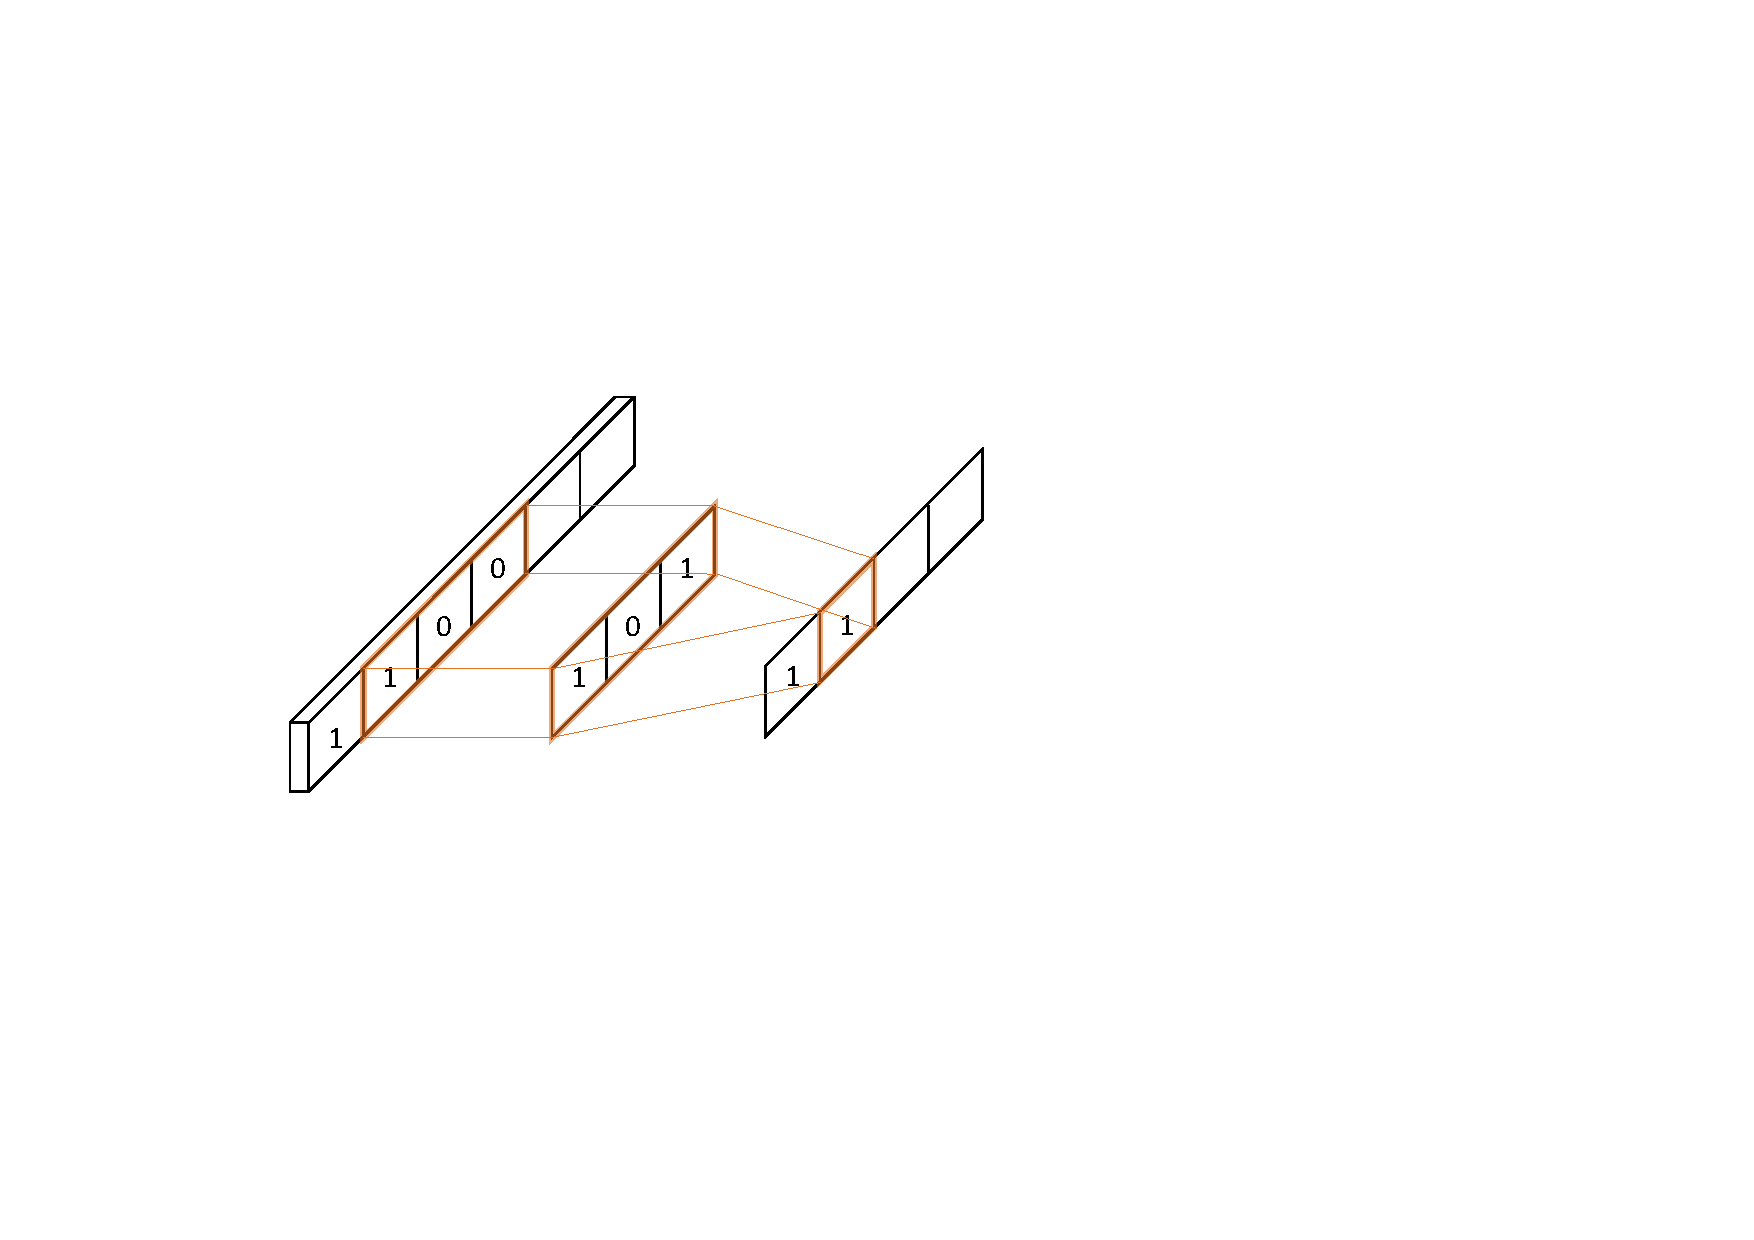
\includegraphics[width=0.4\textwidth]{cnn/kernel_calculation.pdf}
  \caption {Convolution of Input and Kernel based on \cite{Ganesh2019}}
  \label{fig:kernel}
\end{figure}

Compared to regular neural networks CNNs profit a lot from its weight sharing concept. The kernel weights are learned throughout the training. Since the same kernel is applied on different areas of the input, it is not necessary to train a weight for every pixel along the whole spatial dimension of the input. This reduces the number of learnable parameters in the network \cite{OShea2015}. Since the kernel is applied on different areas of locations, the feature search is insensitive to feature location in the image.

\subsection{Convolution Parameters}

The dimension of the input, which is processed by the kernel, is called receptive field. When increasing the receptive field, more global and otherwise more local features of the input are extracted. When defining a CNN architecture, one has to find a trade-off between a model which is complex enough to capture important information from the data and also keep the number of parameters low. Several hyperparameters can be used to reduce or increase the complexity of the model. After a convolutional layer, three hyperparameters can be used to define the width and height of the resulting feature map. 

\subsection{Dilated Convolution}
Dilated convolution, shown in fig.\ref{fig:dilated_cnn}, is the same as regular convolution, but it involves input pixel skipping during the convolutional operation,to cover a larger area of the input. The kernel is applied to an input subspace which does not cover every neighboring pixel. This decreases the spatial dimension of the resulting feature map \cite{Ganesh2019}.

\begin{figure}[H]
  \centering
  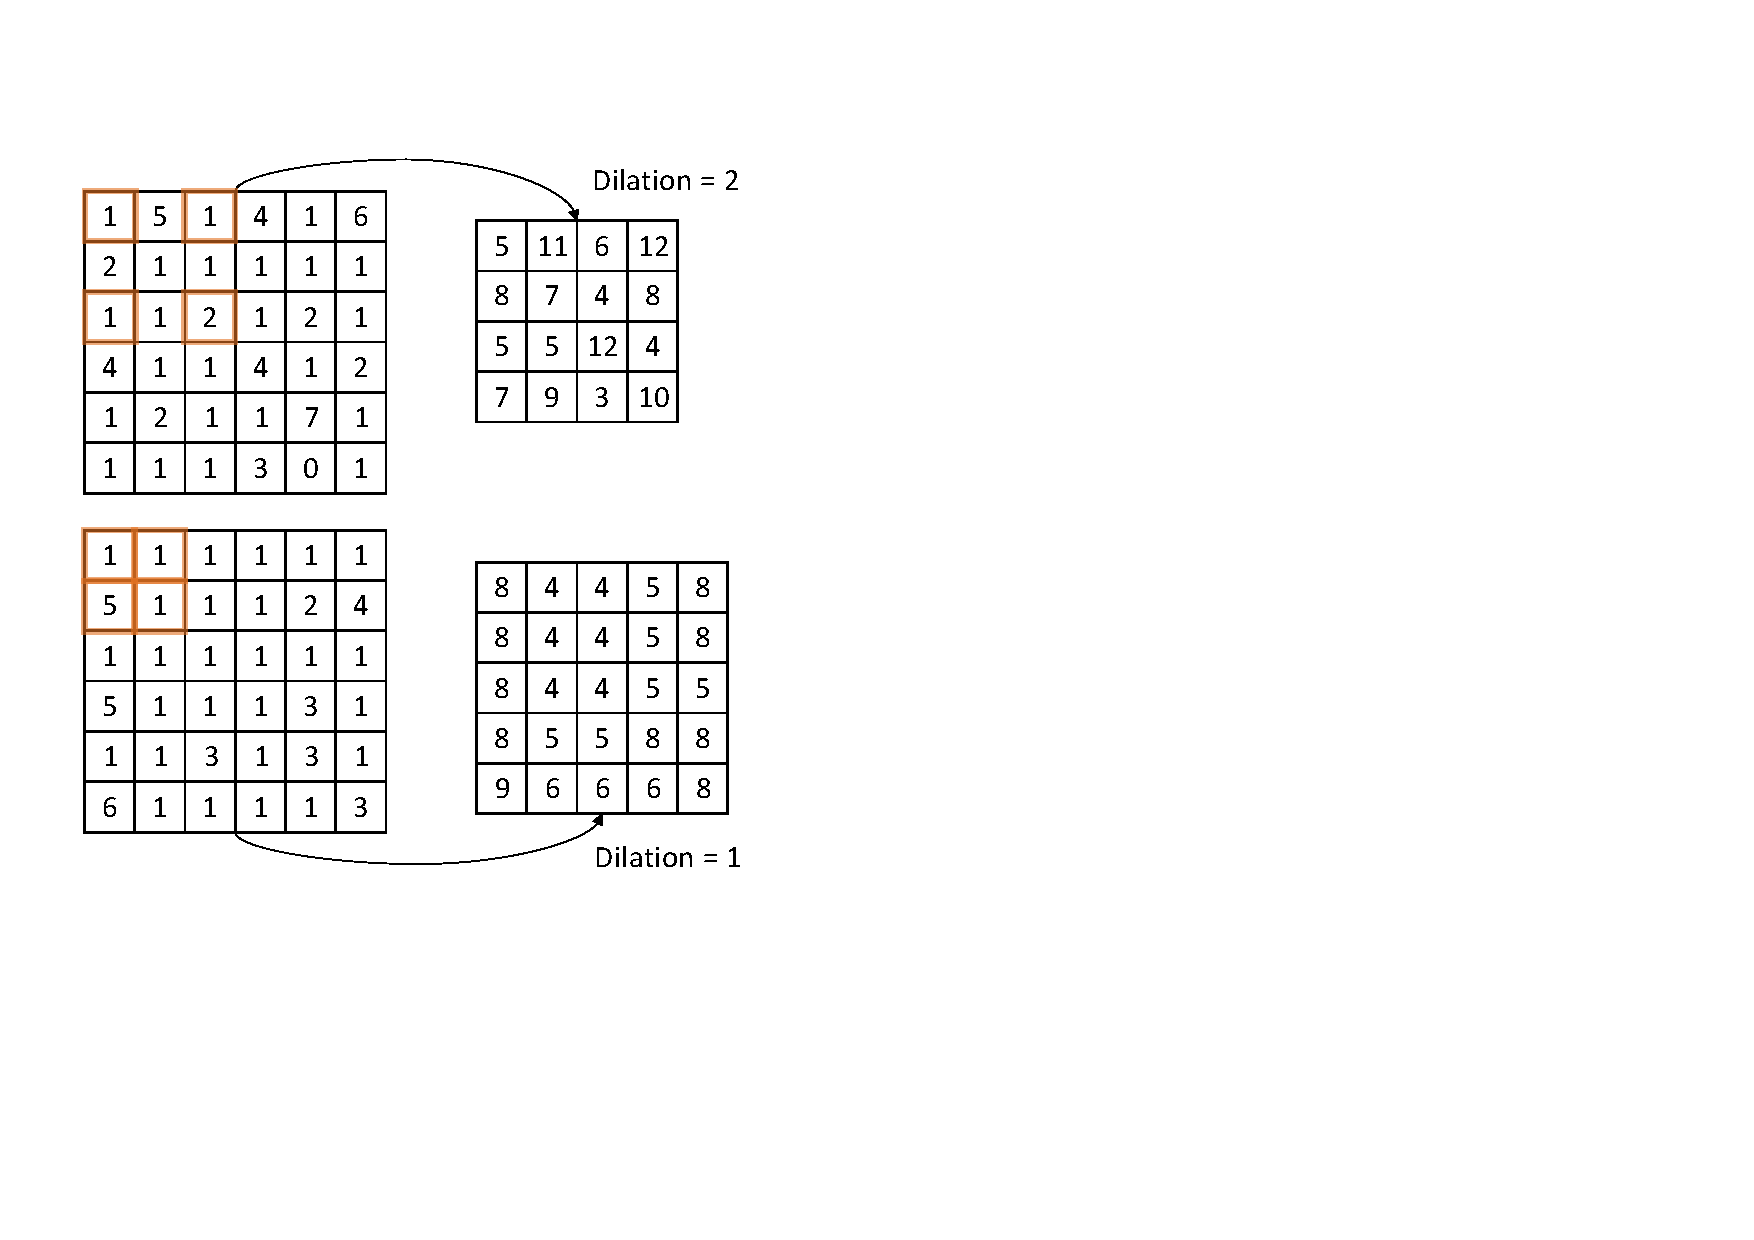
\includegraphics[width=0.4\textwidth]{cnn/dilation_cnn.pdf}
  \caption {Receptive Field for Convolution with Different Dilation Factors}
  \label{fig:dilated_cnn}
\end{figure}


\subsection{Stride}
By increasing the stride, the kernel skips several input pixels while shifting the kernel. The effects of different stride factors are shown in fig.\ref{fig:stride_cnn}. Also, this convolution variant decreases the spatial dimension of the resulting feature map \cite{OShea2015}.

\begin{figure}[H]
  \centering
  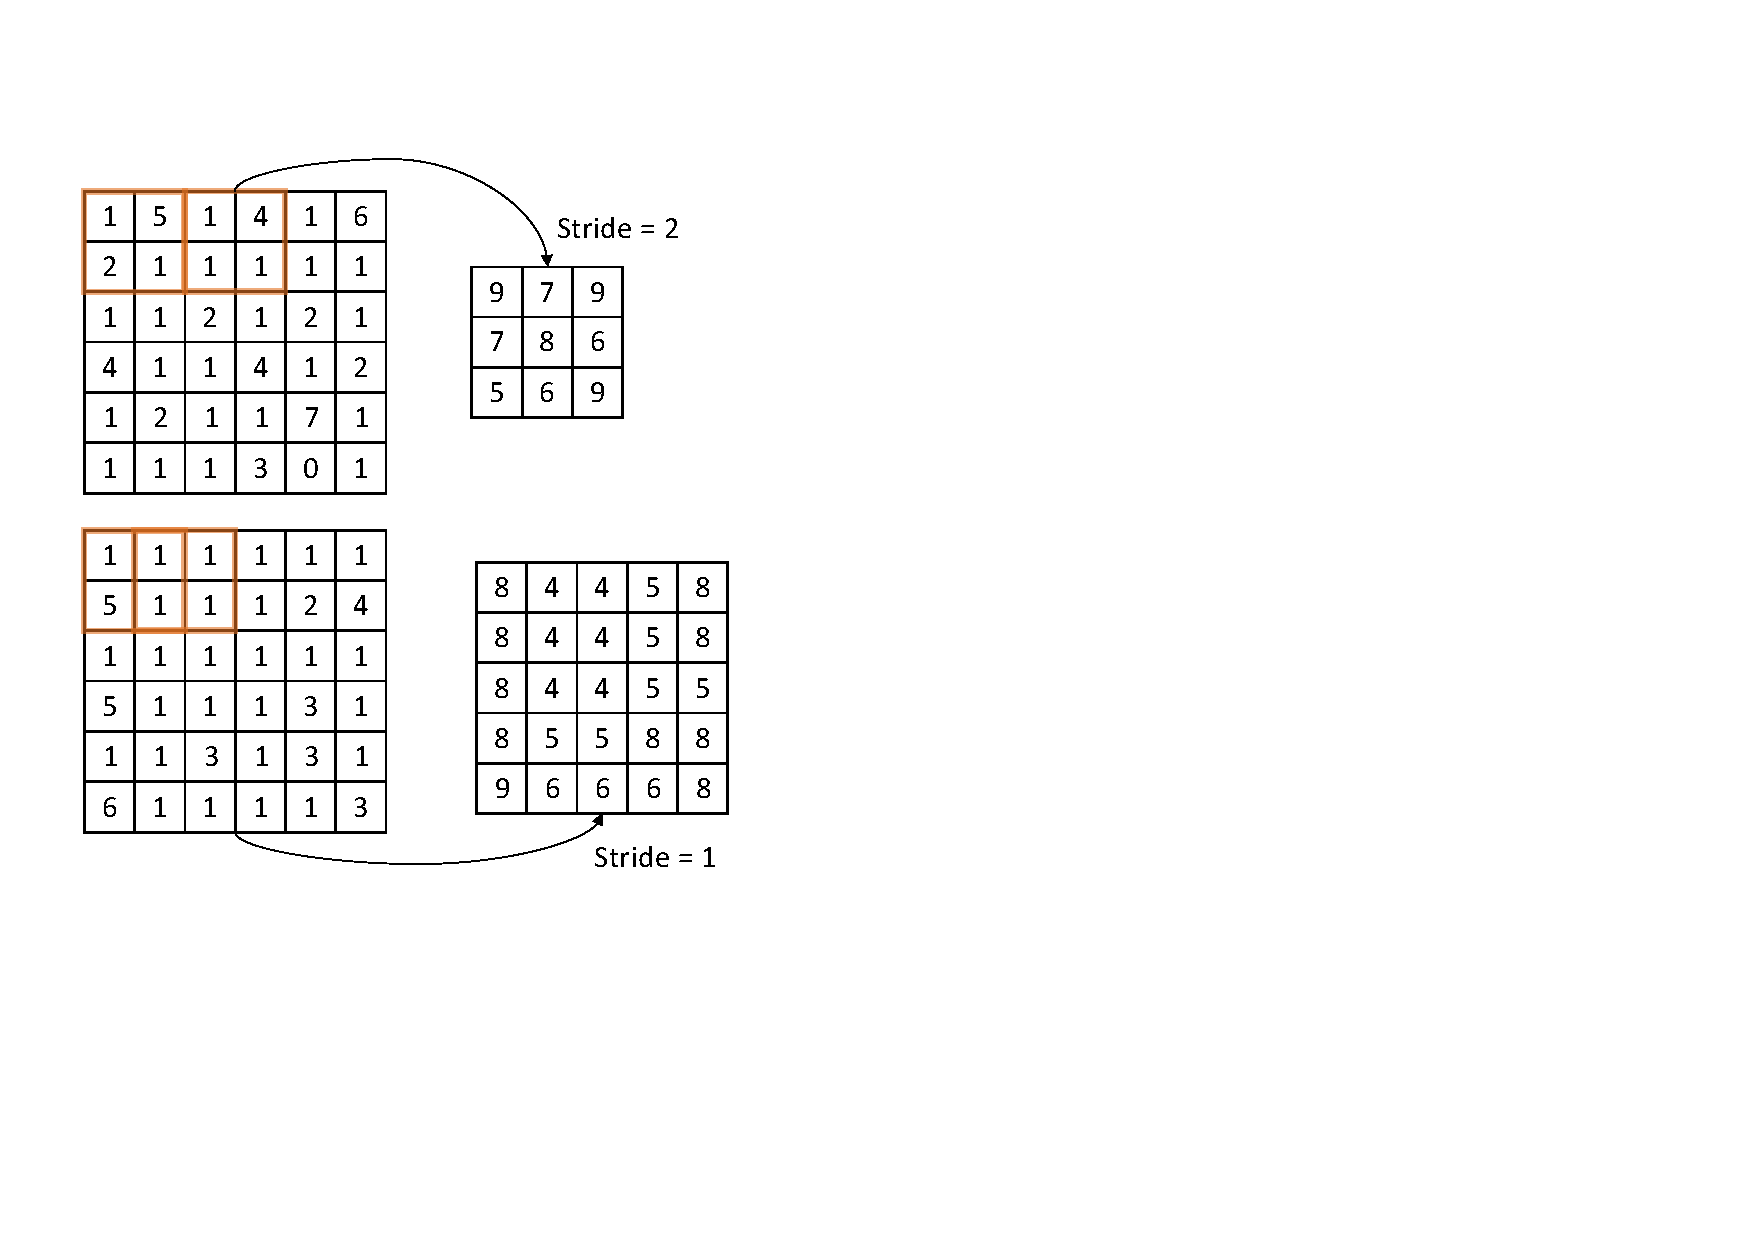
\includegraphics[width=0.4\textwidth]{cnn/stride_cnn.pdf}
  \caption {Convolution with Different Stride Factors}
  \label{fig:stride_cnn}
\end{figure}


\subsection{Zero Padding}
Zero padding, shown in fig.\ref{fig:zero_padding_cnn}, enlarges the input with a border of zeros. During the convolution, the kernel covers an increased spatial dimension of the input, which increases the spatial dimension of the resulting feature map \cite{OShea2015}.

\begin{figure}[H]
  \centering
  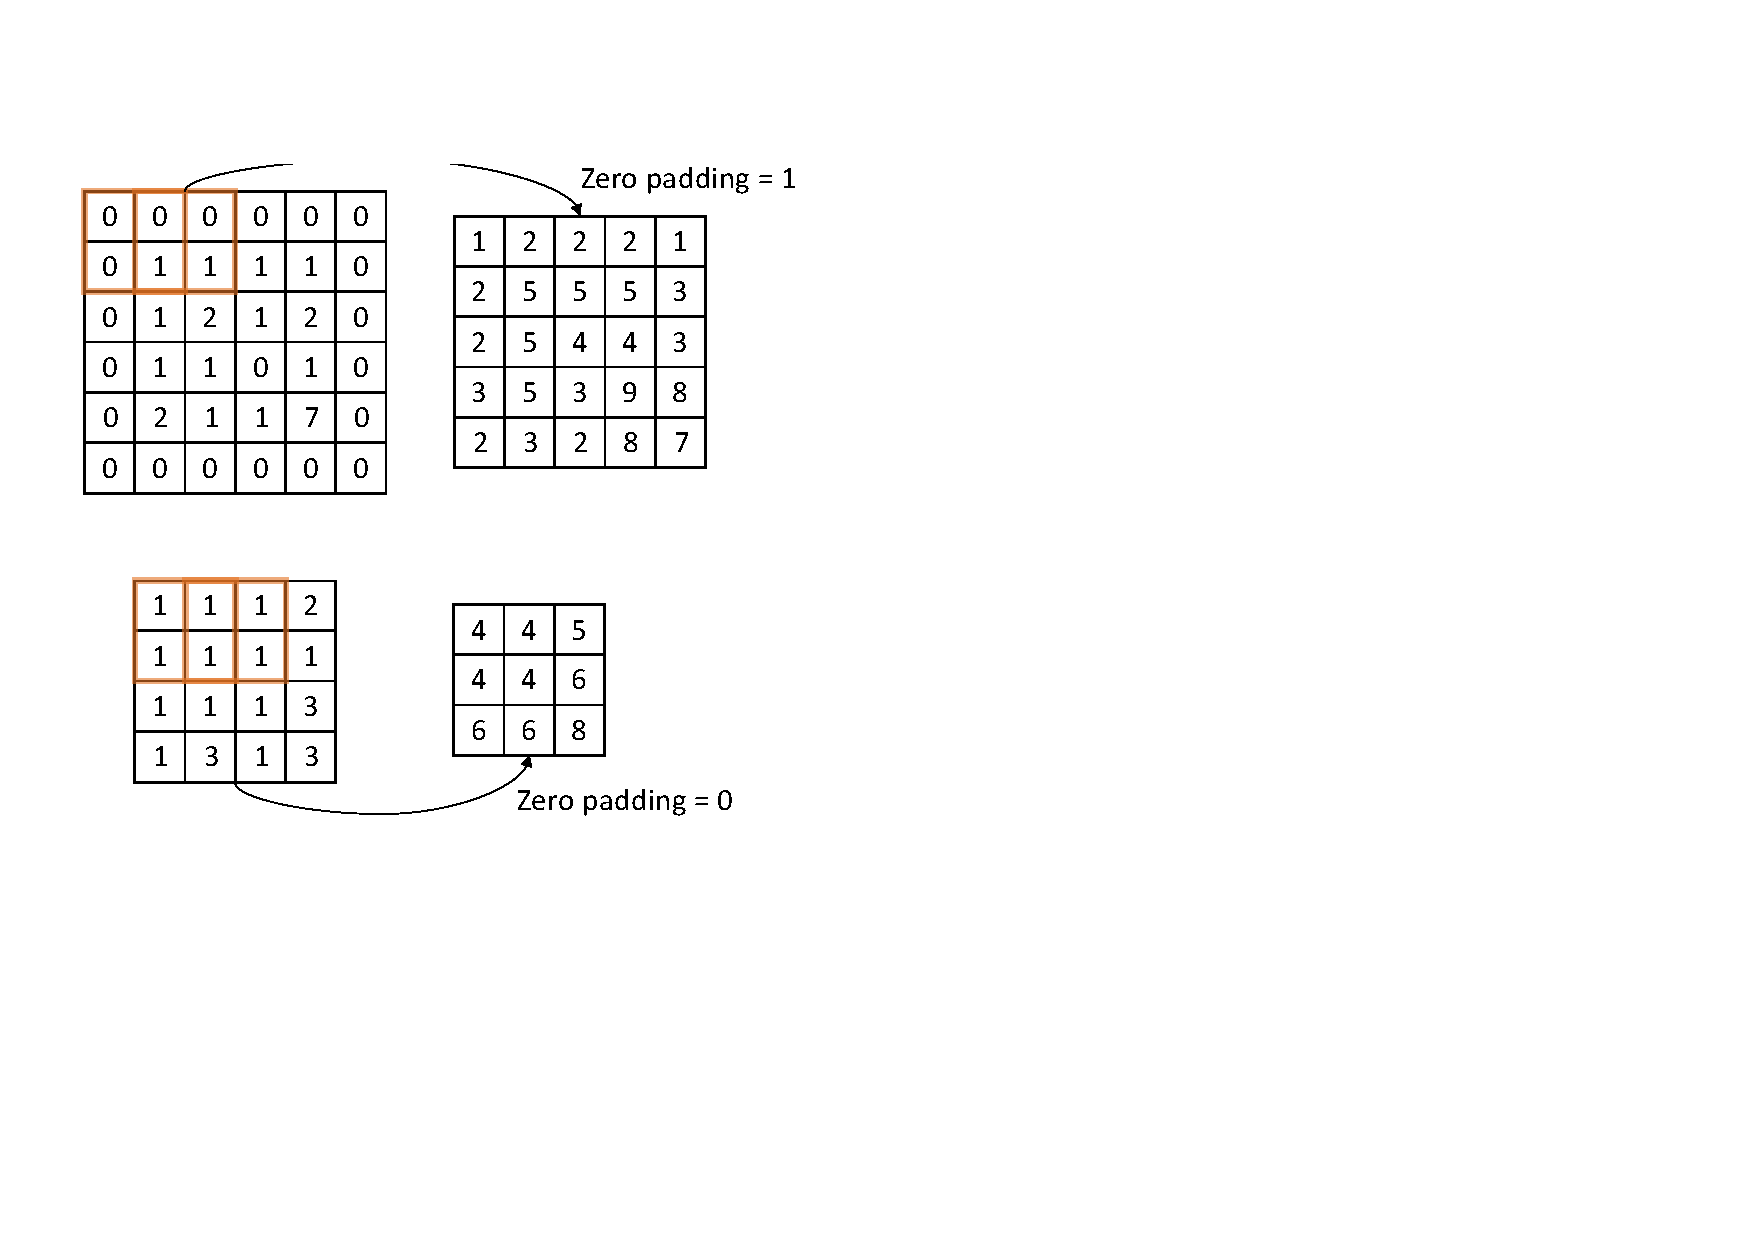
\includegraphics[width=0.4\textwidth]{cnn/zero_padding_cnn.pdf}
  \caption {Convolution with Different Zero Padding}
  \label{fig:zero_padding_cnn}
\end{figure}



\subsection{Spatial Dimension}

 The spatial dimension of the feature map right after a convolutional layer can be calculated as follows:

\begin{equation}
  \frac{(V-R)+2Z}{S+1}, 
  \label{eq:spatial_dimensionality_cnn_feature map}
\end{equation}
where V is the input size, R is the size of the receptive field, Z is the amount of zero padding and S refers to the stride.

\subsection{Pooling Layer}
To change the spatial dimension of the latent feature spaces throughout the network, one can also include pooling layers. There exist different variants like max- and average-pooling. In general, the functionality is similar to convolutional layers with the only difference that no learnable parameters are involved. Also pooling kernels are shifted over the input. For each kernel position, all pixels covered by the kernel are merged to a single value. Max-pooling returns the maximal pixel value and average-pooling the average over all pixels. Often convolutional and pooling layers are applied consecutively \cite{OShea2015}.

\section{Generative Adversarial Network}
Generative Adversarial Networks (GANs) are generative models which recently became more and more popular. Generative models can capture the data distribution of samples seen during training. Such models are able to synthetically generate new instances belonging to the train data distribution without actually being part of that dataset. They can be used in an unsupervised or a supervised manner, which means, they are able to perform feature learning/extraction and classification. GANs include two different models. A generator network (G) learns the data distribution of the training data. Given noise, the generator network produces synthetic data. The discriminator (D) model tries to classify the seen data between synthetic generator's output and true data. D(x) represents the probability that x comes from the real data rather than from the generator. The optimization process of GANs is a minimax game process:
\begin{equation}
    \min_{G} \max_{D} \mathbb{E}_{x \sim P_{r}} [log(D(x))] + \mathbb{E}_{\tilde{x} \sim P_{g}}[log(1-D(\tilde{x}))],
    \label{eq:GAN_Training}
\end{equation}
where $P_{r}$ is the distribution of the real input data and $P_{g}$ is the data distribution from the generator's output, which is defined by  $\tilde{x}  \sim G(z)$. A Uniform or Gaussian distribution can be used to sample the noise $z \sim p(z)$. In theory the generator should be learned such that eq. \ref{eq:GAN_Training} is minimized. This is achieved if the discriminator falsely classifies the real and the synthetic generator's outputs ($D(x) \sim 0$ and $D(\tilde{x}) \sim 1$). On the other hand, the discriminator should be learned such that eq. \ref{eq:GAN_Training} is maximized, which means that the discriminator correctly labels all samples ($D(x) \sim 1$ and $D(\tilde{x}) \sim 0$). The discriminator and generator are optimized in an alternating procedure \cite{Goodfellow2014}. In order to prevent overfitting, one should alternate between k steps of optimizing D and one step of optimizing G \cite{Goodfellow2014}. The optimization of GANs proposed by Goodfellow et al \cite{Goodfellow2014} is described in the Algorithm \ref{alg.GAN_optimization}.

\begin{algorithm}
\caption{Iterative optimization of GANs}\label{alg:cap}
\begin{algorithmic}
\While{$\textrm{train iterations} < \textrm{max iterations}$}
    \While{$\textrm{discriminator optimization steps} < \textrm{k}$}
        \State $\cdot$ Sample m noise samples ${\pmb{z}^{(1)}, . . . , \pmb{z}^{(m)}}$ from noise distribution $p(\pmb{z})$
        \State $\cdot$ Sample m noise samples ${\pmb{x}^{(1)}, . . . , \pmb{x}^{(m)}}$ from real data distribution $P_{r}$
        \State $\cdot$ Update the discriminator by ascending its stochastic gradient:
        \begin{equation*}
            \nabla_{\theta_{d}} \frac{1}{m} \sum_{i=1}^{m} [log(D(\pmb{x}^{(i)})) + log(1-D(G(\pmb{z}^{(i)})))].
        \end{equation*}
    \EndWhile
    \State $\cdot$ Sample m noise samples ${\pmb{z}^{(1)}, . . . , \pmb{z}^{(m)}}$ from noise distribution $p(\pmb{z})$
    \State $\cdot$ Update the generator by descending its stochastic gradient:
    \begin{equation*}
        \nabla_{\theta_{g}} \frac{1}{m} \sum_{i=1}^{m} log(1-D(G(\pmb{z}^{(i)}))).
    \end{equation*}
\EndWhile
\label{alg.GAN_optimization}
\end{algorithmic}
\end{algorithm}

Besides that, eq. \ref{eq:GAN_Training} does not deliver sufficient gradients for gradient-based optimization of GANs. The problem is, that in early stages the generator performance is poor, such that the discriminator rejects all synthetic generator's outputs, which prevents the generator training. Instead, the generator can be trained to maximize $D(\tilde{x})$. This objective achieves the same results as eq. \ref{eq:GAN_Training} but delivers stronger gradients in early learning stages \cite{Goodfellow2014}. Fig \ref{fig:GAN_training_vizualization} shows the alternating optimization of the discriminator and generator. 

\begin{figure}[p]
  \centering
  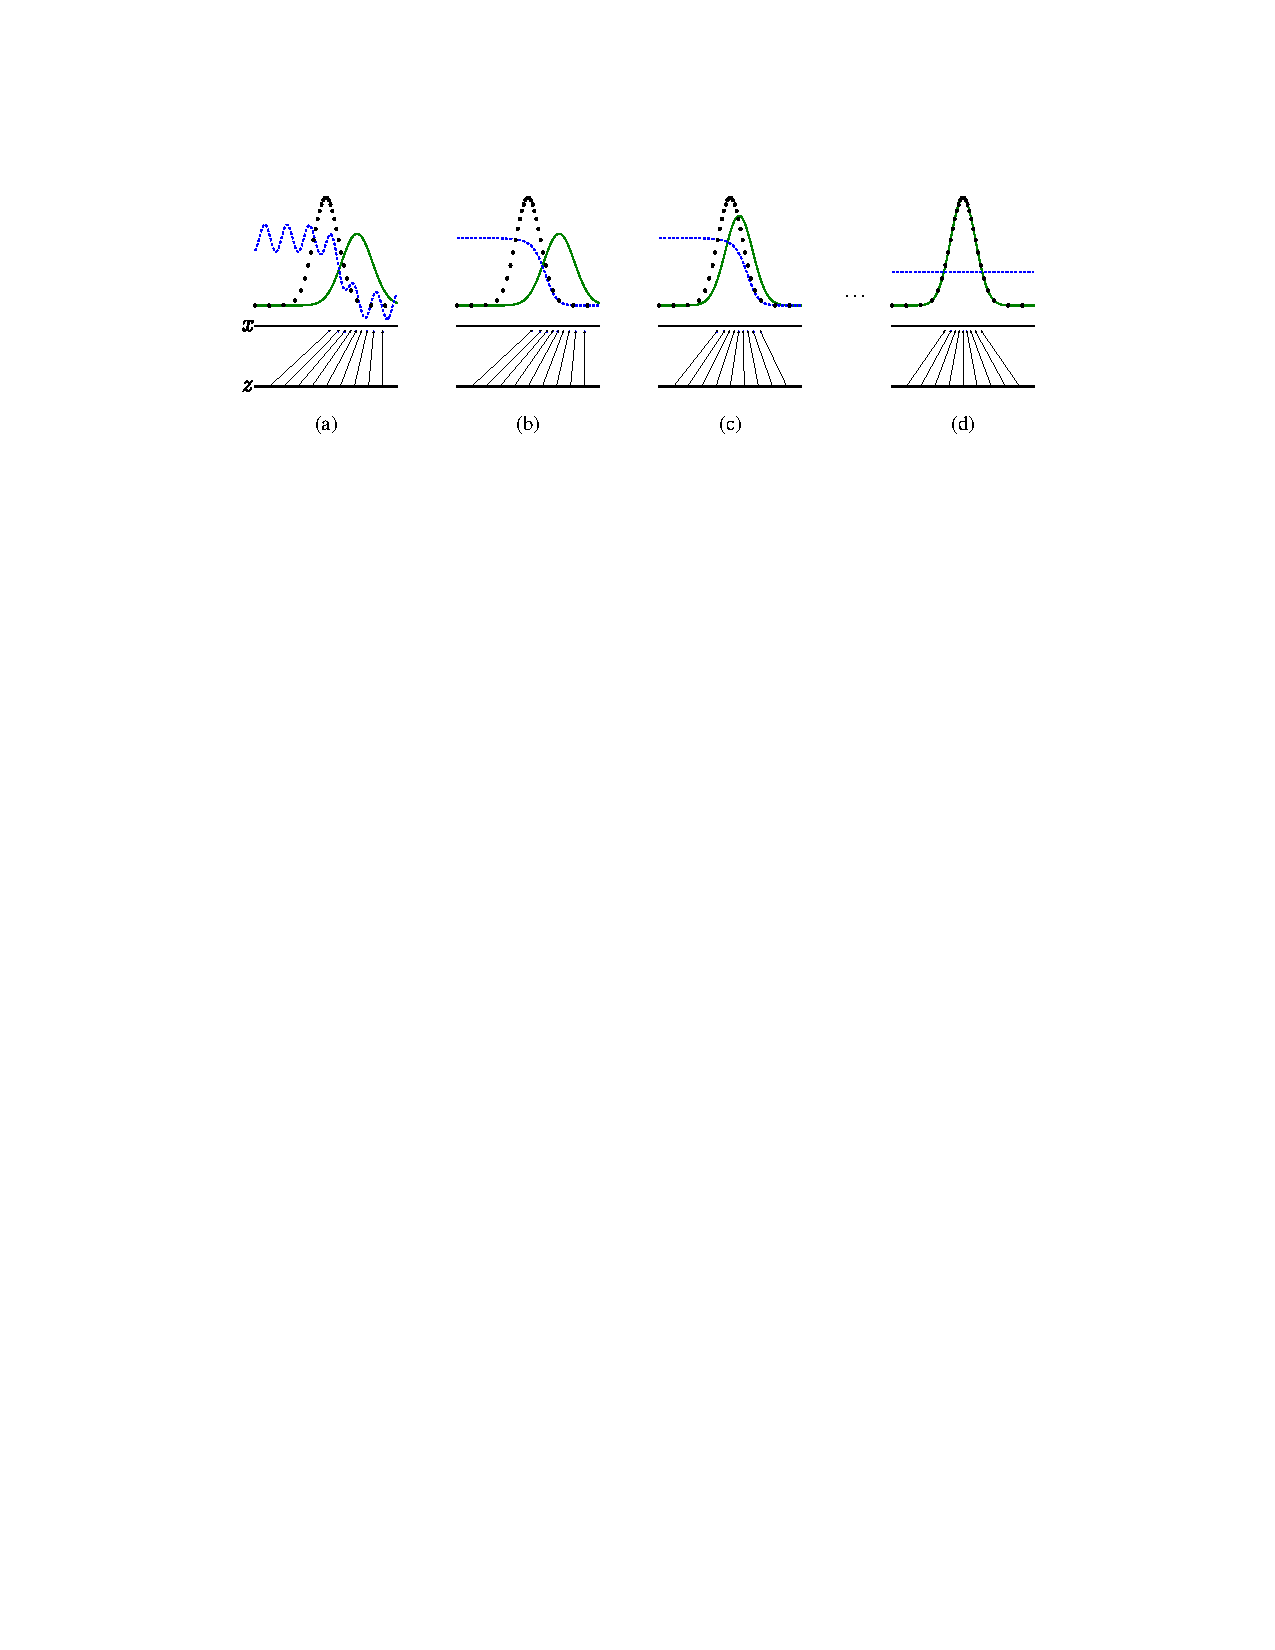
\includegraphics[width=1\textwidth]{GAN_training_vizualization.pdf}
  \caption{When optimizing GANs the discriminator and generator are optimized simultaneously in an alternating procedure. The blue dashed line represents the discriminator probability of x belonging to the real data distribution rather than being created by the generator. The black dashed line represents the generative distribution and the green solid line the real data distribution. (a) shows a generator, discriminator pair near convergence, (b) shows the GAN performance after passing the inner loop of Algorithm \ref{alg.GAN_optimization}, which optimizes the discriminator. (c) shows the GAN performance after passing through one whole training loop in Algorithm \ref{alg.GAN_optimization}. Now the generator and the discriminator are both optimized. (d) shows the GAN performance after several training iterations. The generator completely learned the real data distribution, such that the discriminator is not able to separate between samples from the real data distribution and synthetic generator outputs \cite{Goodfellow2014}.}
  \label{fig:GAN_training_vizualization}
\end{figure}

\section{Deep Belief Network}

Deep belief networks (DBNs) are generative models, which contain stacked Restricted Boltzmann machines (RBMs), which are widely used in research and industry.

\subsection{Restricted Boltzmann Machine}
RBMs consist of hidden and visible layers, each containing several units. DBNs use RBMs, which are a variation of regular Boltzmann machines with the restriction that it's units must form a bipartite graph. This requires that all RBM units are separated in two disjoint and independent subsets (hidden and visible subset). Visible and hidden units are connected through weighted connections, but not the units belonging to the same layer. The units in the hidden and visible layer are binary. The matrix $W \in \mathbb{R}^{mxn}$ contains all the weights for connecting the m nodes of the hidden and n nodes of visible unit and $a \in \mathbb{R}^{m}$ and $b \in \mathbb{R}^{n}$ include the biases of the hidden and visible unit \cite{Hinton2010}. The connection of the visible and hidden unit is visualized in \ref{fig:RBM}. RBMs are energy-based models. For each combination of visible $\mathbf{v}$ and hidden layer units $\mathbf{h}$ the energy is calculated as following:

\begin{equation}
\begin{aligned}
    E(v,h) = -\sum_{i \in visible} a_{i}v_{i}-\sum_{j \in hidden} b_{j}h_{j}-\sum_{i,j} v_{i}h_{j}w_{ij},
\end{aligned}
\end{equation}
where $v_{i}$, $h_{j}$ are the binary states of the i-th and j-th unit in the visible and hidden layer. $a_{i}$, $b_{j}$ and $w_{ij}$ are the biases and weights corresponding to the i-th unit in the visible and the j-th unit in the hidden layer. Based on this energy, the network assigns a probability to every possible combination of visible and hidden layer units:

\begin{equation}
\begin{aligned}
    p(\mathbf{v,h}) = \frac{1}{Z} e^{-E(\mathbf{v,h})},
\end{aligned}
\end{equation}
where Z is a "partition function", which sums up the probabilities of all hidden and visible unit combinations. Z normalizes $p(\mathbf{v,h})$ to a value between 0 and 1:

\begin{equation}
\begin{aligned}
    Z = \sum_{\mathbf{v,h}}e^{-E(\mathbf{v,h})}.
\end{aligned}
\end{equation}

The network assigns a probability for each visible unit by summing up $p(\mathbf{v,h})$ for all possible hidden vectors:
\begin{equation}
\begin{aligned}
    p(\mathbf{v}) = \frac{1}{Z} \sum_{h} e^{-E(\mathbf{v,h})}.
    \label{eq:prob_visible_layer}
\end{aligned}
\end{equation}

Since the units of RBMs must form a bipartite graph, there are no connection between two hidden or visible units. Given a training sample, the visible units can be calculated with eq. \ref{eq:prob_visible_layer}. From there, the hidden units can be calculated as following:
\begin{equation}
\begin{aligned}
    P(h_{i}|v) = \sigma(b_{j} + \sum_{i=1}^{n} W_{i,j} v_{i}).
    \label{eq:prob_hidden_layer}
\end{aligned}
\end{equation}
where $h_{j}$ is the j-th unit in the hidden layer and $v_{i}$ the i-th unit in the visible layer. Afterwards the units of the visible layer can be reconstructed as following:
\begin{equation}
\begin{aligned}
    P(v_{i}|h) = \sigma(a_{i} + \sum_{j=1}^{n} W_{i,j} h_{j}),
    \label{eq:prob_reconstructed_visible_layer}
\end{aligned}
\end{equation}
This iterative RMB training is separated in two phases. The positive phase is the one where the hidden units are updated based on the visible units, which is defined in eq. \ref{eq:prob_hidden_layer}. In the negative phase, which is defined in eq. \ref{eq:prob_reconstructed_visible_layer}, the visible units are reconstructed based on the previously calculated hidden units. This process is also visualized in fig. \ref{fig:RBM}. The weights and biases of the network can be updated such that the reconstruction error is minimized:

\begin{equation}
\begin{aligned}
    \Delta w_{ij} = \epsilon(\langle v_{i}, h_{j}\rangle_{data}- \langle v_{i}, h_{j}\rangle_{reconstructed}), 
    \label{eq:RBM_weight_update}
\end{aligned}
\end{equation}
where the angle brackets denote expectations under the distribution specified in the subscripts. The subscript $data$ refers to the expectation of the train dataset and subscript $reconstructed$ to the expectation of the defined model. A better training is achieved if more steps of alternating visible and hidden layer updates are performed before collecting the statistics for the second term $\langle v_{i}, h_{j}\rangle_{reconstructed}$ in the learning rule \cite{Hinton2010}.

\begin{figure}[H]
  \centering
  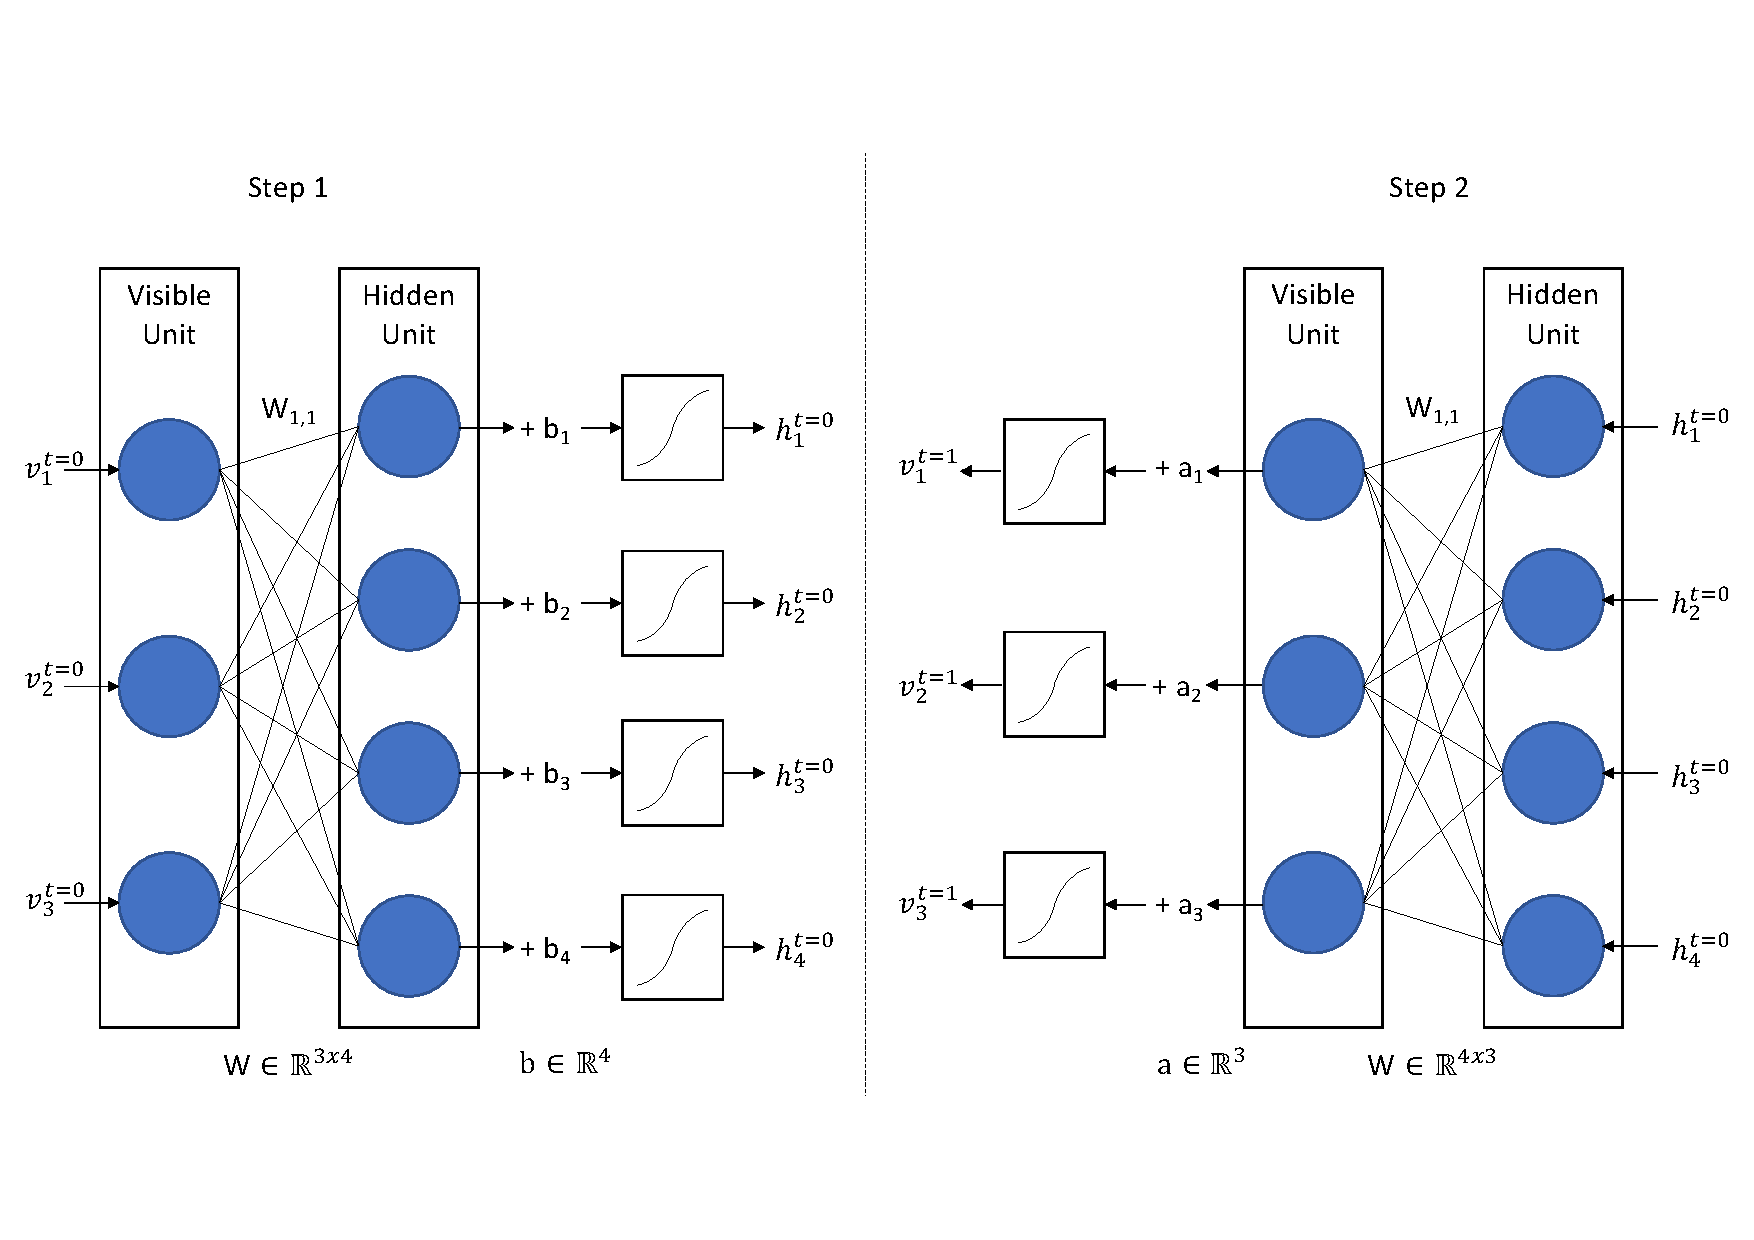
\includegraphics[width=1\textwidth]{RBM.pdf}
  \caption {Optimization of RBM} \label{fig:RBM}
\end{figure}


RBMs are generative models which make guesses about the probability distribution of the original input. By training the RBM the divergence between the true input distribution and the reconstructed ones is minimized \cite{Hinton2010}.

\subsection{Training Deep Belief Network}
As shown in fig. \ref{fig:DBN} DBNs connect several RBMs in a specific order. The units of the visible and hidden layer of the first RBM are updated by applying the positive and negative phase in an alternating manner. The hidden layer of this RBM is treated as visible layer for the consecutive RBMs. This greedy learning algorithm is applied until all RBMs in the DBN are trained. After this layer to layer update is completed, the supervised training of the DBN is started. The backpropagation training considers all layers simultaneously while updating weights and biases to increase the classification accuracy of the DBN \cite{Zhang2017}.

\begin{figure}[H]
  \centering
  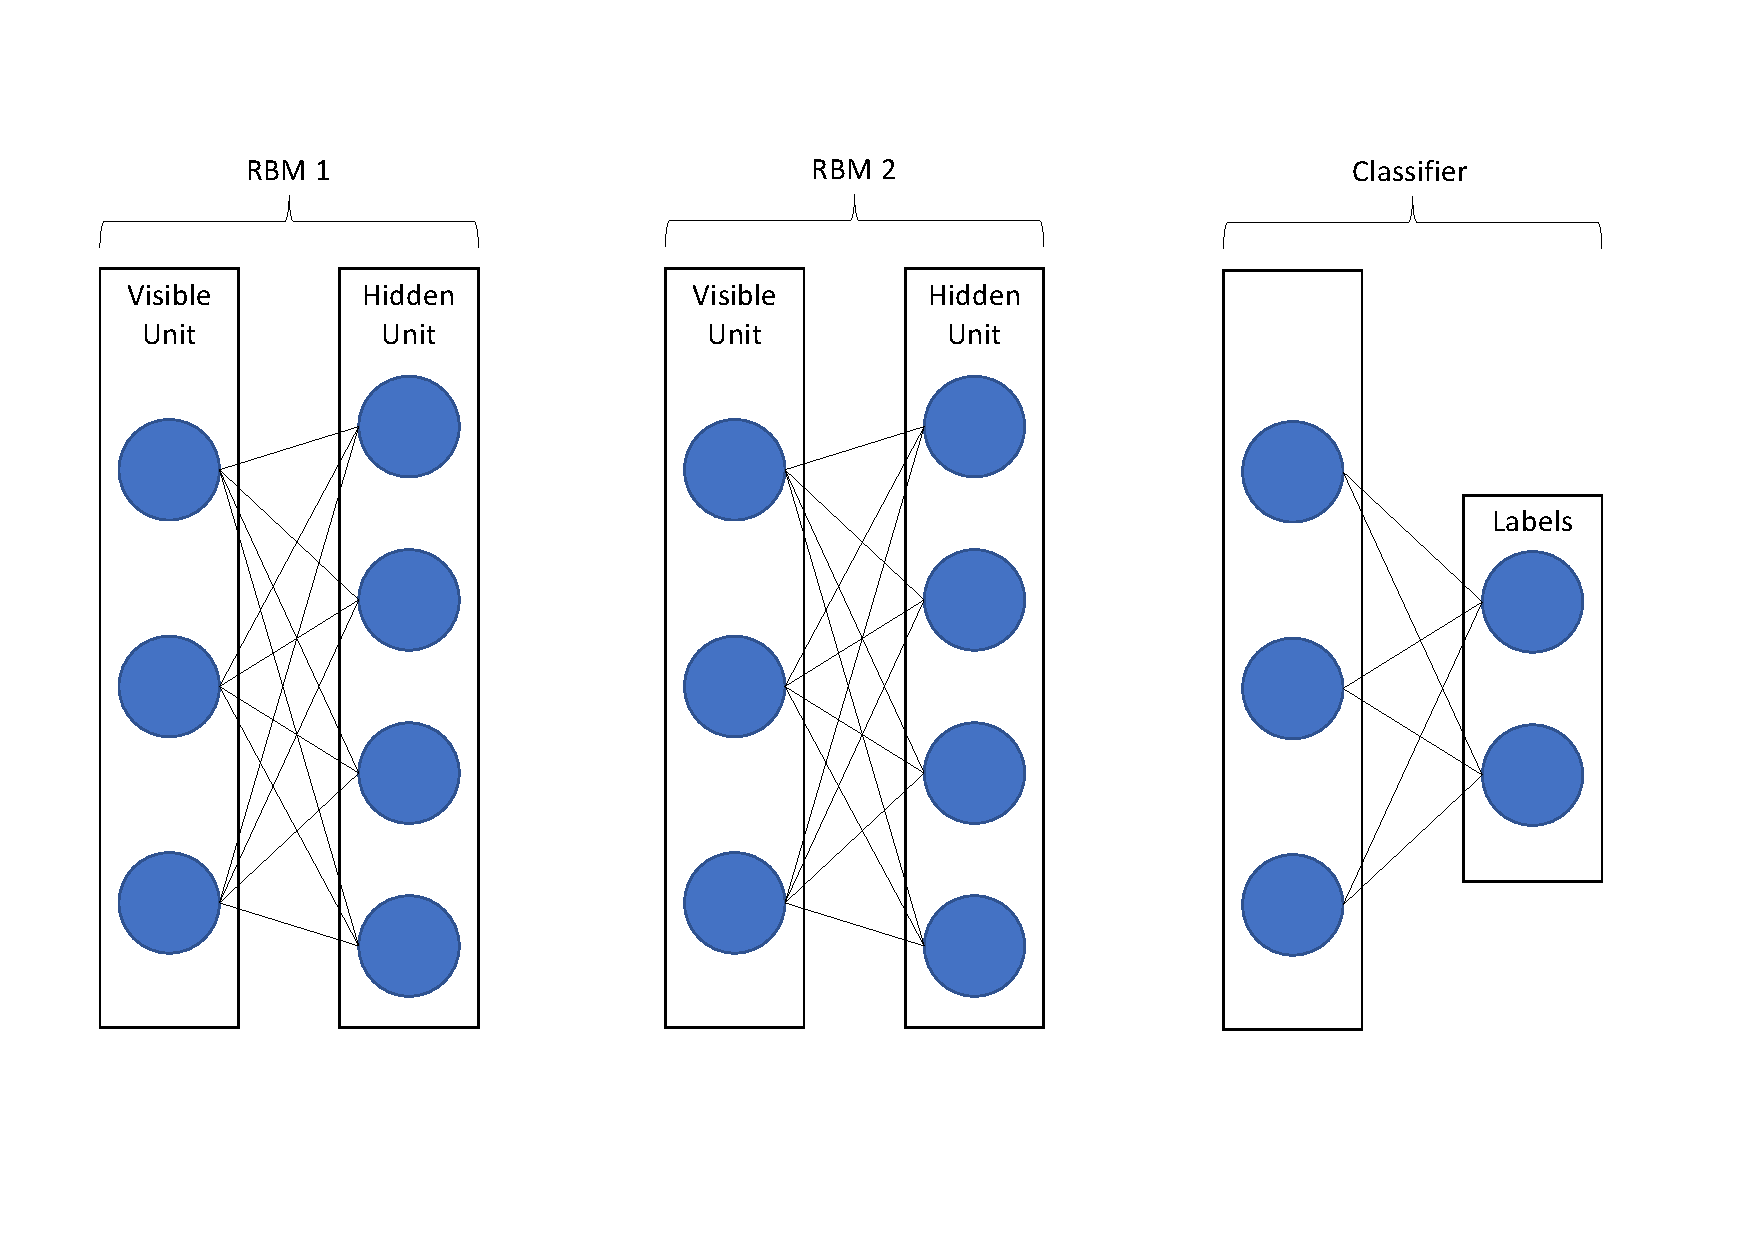
\includegraphics[width=1\textwidth]{DBN.pdf}
  \caption {Structure of DBN based on \cite{Zhang2017}} \label{fig:DBN}
\end{figure}


\section{Domain Adaptation and Transfer Learning}

In the computer vision community, domain adaption and transfer-learning techniques recently received more and more attention. Transfer learning, also called multi-task learning, is a problem related to domain adaption. The goal is to train a model to solve a specific task on a given dataset. The model should then be used to solve a different task on the same data. The data used in the tasks is equally distributed, but in different tasks the relation between samples and ground truth outputs differs. For this reason, the conditional distribution differs, whereas the marginal distribution is the same for the different tasks. Domain adaption refers to problems in which a model is trained on labeled train data, denoted as source domain. The model is then applied to solve an equal task on the unlabeled test data, denoted as target domain. The target and source domain data come from different distributions, anyhow the data must be related in any sense and structured similarly. The conditional and marginal distribution for the source and target domain data differ. Generally, one can say domain adaption is used to reduce the discrepancy between data distributions. In this sense, a model is trained to solve the same task on differently distributed data. Transfer learning on the other hand learns a model, which is able to solve different tasks on the same dataset. The differences are visualized in fig. \ref{fig:domain_adaption_vs_transfer_learning}

\begin{figure}[H]
  \centering
  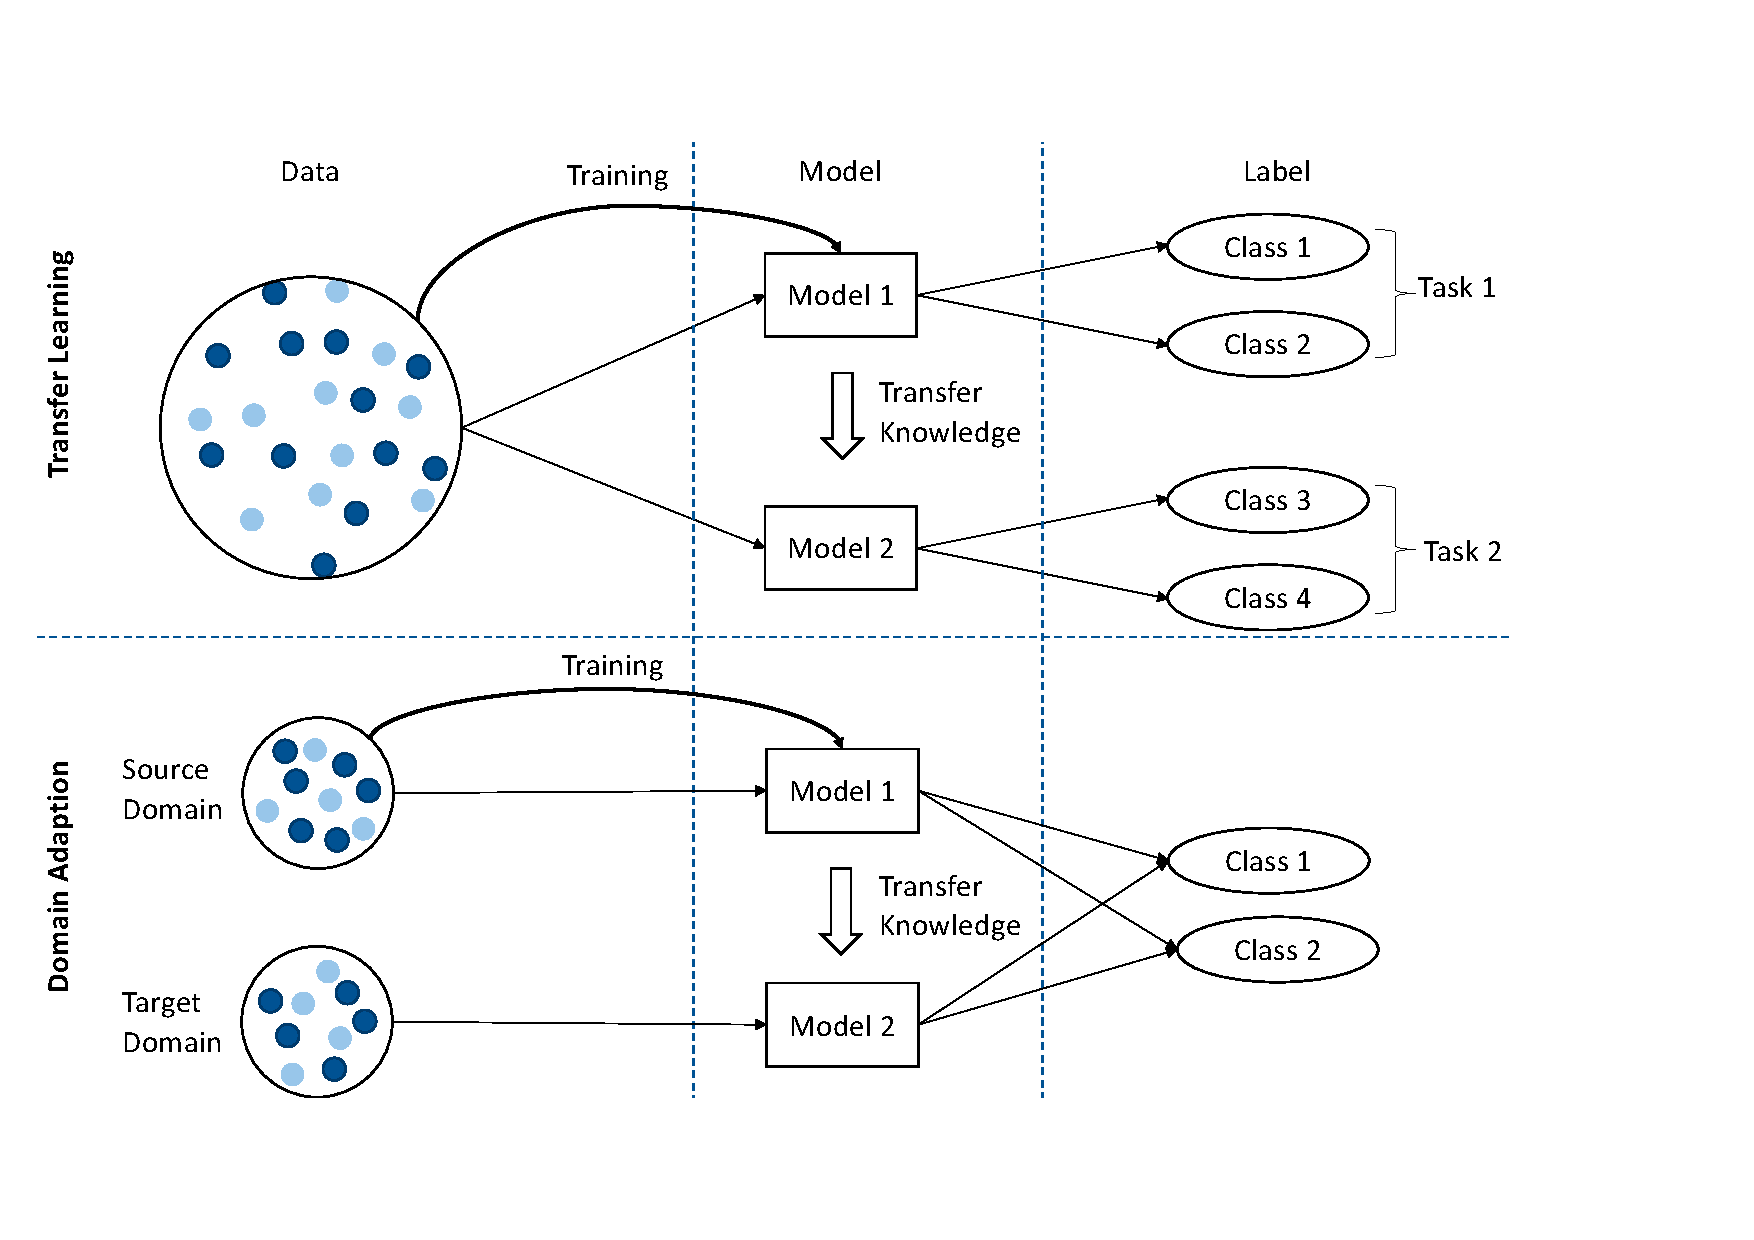
\includegraphics[width=.8\textwidth]{domain_adaption_vs_transfer_learning.pdf}
  \caption {Transfer Learning vs. Domain Adaption} \label{fig:domain_adaption_vs_transfer_learning}
\end{figure}


Since the focus of this thesis is to analyze domain adaption approaches, the following passages explain the different aspects of domain-adaption.
\subsection{Notation}
The labeled source domain data is denoted by  $S = {(x_{i}^{s}, y_{i}^{s})_{i = 0}^{i = N_{s}}}$. Generally, the target domain data is separated in labeled $T_{l} = {(x_{i}^{tl}, y_{i}^{tl})_{i = 0}^{i = N_{tl}}}$ and unlabeled data $T_{u} = {(x_{i}^{tu})_{i = 0}^{i = N_{tu}}}$. Usually, it is assumed that there is a large amount of labeled data in the source and a small amount of labeled data in the target domain: $N_{tl} \ll N_{s}$. In this conext $x_{i}$ is referred as the observation and $y_{i}$ as the corresponding label  \cite{Patel2015}. Depending on the data available during training, one differs between different branches of domain adaption: 
\begin{itemize}
\item \textbf{Semi-supervised Domain Adaptation}, where a function is trained to use the data from $S$, $T_{l}$
\item \textbf{Unsupervised Domain Adaptation}, where a function is learned using the data from $S$ and $T_{u}$ \cite{Patel2015} 
\end{itemize}

From a statistical point of view, the source and target domain can be described by the marginal distribution $P(X)$ and conditional distribution $P(Y|X)$. It is required that the data from source and target have the same data space and label space, but the marginal and conditional distribution may differ $P(Y_{s}) \neq P(Y_{t})$ and $P(Y_{s}|X_{s}) \neq P(Y_{t}|X_{st})$ \cite{Qikang2020}

\subsection{Types of Transfer Learning}
Generally, domain adaption approaches can be grouped in four different types \cite{AZAMFAR2020103932}:  

\begin{itemize}
\item \textbf{Instance Weighting Methods} can be used to address this covariate shift problem by integrating weights into a loss function that estimates the discrepancy between source and target. Weighting factors like $\frac{P_{t}(x)}{P_{s}(x)}$ can be used. When a source domain sample has a high probability to be in the target domain, this means that the source domain sample is quite similar to the target domain samples. Samples like that should be strongly included in the training to optimize the model to work well on the target domain data.
\item \textbf{Feature-Based Transfer Learning} has the goal to find a feature space in which the domain discrepancy is reduced. All source and target samples are transferred in the domain-invariant feature space, where the classification of data from both domains works well. Fig. \ref{fig:Domain_adaption_intro} illustrates how feature-based domain adaption can be used to find a cross-domain classifier which accurately separates source and target domain data \cite{Pandhare2021}. 
\item \textbf{Model-Based Transfer Learning} aims to find a classifier trained on the source domain, which can be transferred or fine-tuned to perform well on the target domain.
\item \textbf{Relation-Based Transfer Learning} has the goal to find and utilize similarities between the two domains, which helps to transfer knowledge. 
\end{itemize}

\begin{figure}[H]
  \centering
  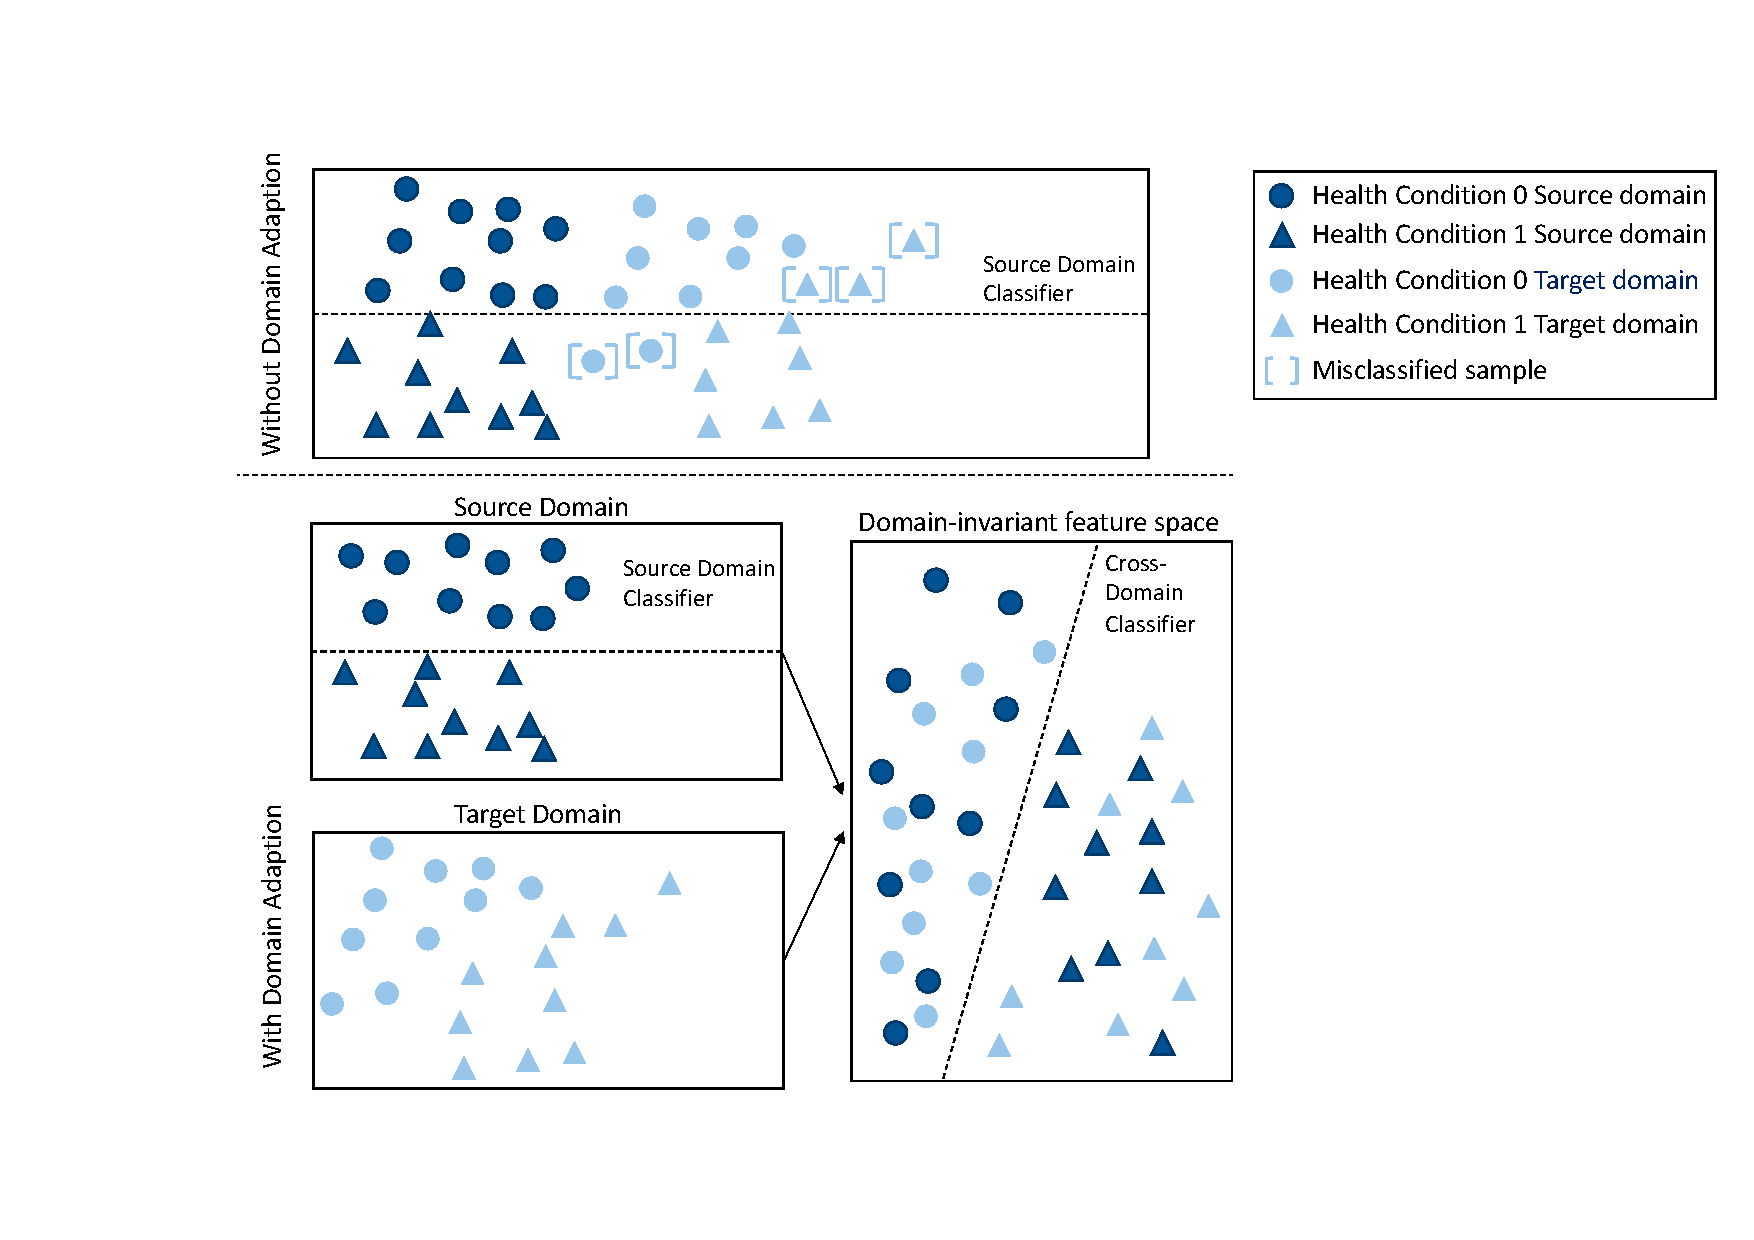
\includegraphics[width=1\textwidth]{domain_adaption_intro.pdf}
  \caption {Domain Adaption for Health Monitoring of Machines with Different Working Conditions based on \cite{Pandhare2021}} \label{fig:Domain_adaption_intro}
\end{figure}


\section{Maximum Mean Discrepancy}
Maximum Mean Discrepancy (MMD) is a criterion which estimates the discrepancy between two distributions. MMD can be used to optimize a neural network such that the distribution discrepancy in its latent feature space is reduced. In the reproducing kernel Hilbert space (RKHS) the discrepancy is measured as squared distance between the distribution kernel embeddings. The distribution discrepancy across domains can be measured in several layers of the neural network. Including this information in the optimization of the model helps to avoid feature transferability degradation. Anyhow, one has to pay attention to not transfer noise or irrelevant information, since this destroys the structure of the source and target domain data and makes the classification task even more difficult \cite{li2020}. 

\begin{align}
    M_{k}(P,Q) = \Bigl|  \boldsymbol{E_{P}}[\Phi(\boldsymbol{X^{s}})] - \boldsymbol{E_{Q}}[\Phi(\boldsymbol{X^{t}})]     \Bigl|^{2}_{Hk}
\end{align}

Hk denotes the RKHS, which is described by the characteristic kernel k and the mapping function $\Phi$. When taking the identity function as mapping function, the discrepancy of the distribution means is measured. When using more complex mapping functions also higher order moments can be matched \cite{Yujia2015}. The distributions of the source domain $X^{s} = \{{x}_{i}^{s}\}_{i=0,...,n_{s}}$ and target domain $X^{t} = \{{x}_{i}^{t}\}_{i=0,...,n_{t}}$ in the latent feature space of interest are represented by P and Q. $\boldsymbol{E_{P}[.]}$ is the expected value of the source distribution and $\boldsymbol{E_{Q}[.]}$. The kernel choice is of great importance when applying MMD for optimizing neural networks. For this reason, it makes sense to combine several kernels to profit from their individual performance:

\begin{align}
    k(\boldsymbol{X^{s}}, \boldsymbol{X^{t}}) = \sum_{i=0}^{N_{k}} k_{\sigma_{i}}(\boldsymbol{X^{s}}, \boldsymbol{X^{t}})
\end{align}

$N_{k}$ denotes the number of kernels used in the RKHS and $k_{\sigma_{i}}$ represents one individual RBF kernels  \cite{li2020}. Other kernels like linear kernels could be used, but current research shows that RBF kernels usually perform best \cite{AZAMFAR2020103932}.
